\chapter{نتیجه‌گیری}
نتایج آزمایش‌های انجام‌شده با استفاده از ابزار توسعه داده شده در نمودارها و جدول‌های متفاوت گردآوری شده‌اند. دسته‌بندی این نتایج در حالت‌های متفاوت و با دیدگاه‌های مختلف در بخش‌های این فصل تدوین‌شده تا خواننده بتواند بر اساس آن‌ها قضاوت منصفانه‌تری را داشته باشد.

\section{روند آزمایش‌ها}
همان‌طور که در قبل هم اشاره شد، انجام آزمایش‌ها روندی الگوپذیر بوده است. برای بهبود و تسریع در این روند، از ابزار اشاره شده در طول آزمایش‌ها بهره‌برداری شده است.

آزمایش‌ها به این صورت بوده که برای هر پلتفرم، پیاده‌سازی الگوریتم‌های محک، به صورتی که این پیاده‌سازی‌ها از یک ساختار الگوریتمی و نرم‌افزاری یکسان پیروی کنند، انجام شده است. این که ساختار در پیاده‌سازی‌های مختلف حفظ شود به این معنا است که مثلاً اگر در پیاده‌سازی یک الگوریتم در یک پلتفرم نیاز است از حلقه استفاده شود، در دیگری هم به همین صورت باشد به‌طوری‌که در هر دو پلتفرم پیاده‌سازی‌ها از پیچیدگی محاسباتی یکسانی برخوردار باشند چرا که هدف محک منصفانهٔ آن‌ها است. برای این امر، وقت زیادی از پژوهش صرف شد چرا که پیاده‌سازی‌های موجود در هر پلتفرم با دیگری متفاوت است و عملاً برای محکی که جانب انصاف را رعایت کند، نمی‌تواند مورداستفاده قرار بگیرد. در نتیجه در پیاده‌سازی‌های موجود باید تجدید نظر انجام می‌شد.

همان‌طور که اشاره شد، هدف  پژوهش ما کاربرانی بوده‌اند که از رایانه‌های شخصی استفاده می‌کنند. به همین منظور، رایانهٔ استفاده شده در طول این آزمایش‌ها، رایانهٔ شخصی موجود در آزمایشگاه دانشکده با پردازندهٔ 
\lr{Intel(R) Core(TM) i7-3770 CPU @ 3.40GHz}
با ۸ هستهٔ پردازشی، حافظهٔ ۱۶ گیگابایتی، بدون پردازندهٔ گرافیکی و سیستم‌عامل لینوکس، توزیع اوبونتو با نسخهٔ هستهٔ
\lr{5.15.0-119-generic}
بوده است.


برای آزمایش هر شبیه‌ساز توسط ابزار توسعه داده شده، زمان اجرا و میزان حافظهٔ مصرفی با افزایش تعداد کیوبیت اندازه‌گیری و در پایگاه‌داده ذخیره شده است. از آن‌جایی که شبیه‌سازها در دو پلتفرم Qiskit و Cirq قرار دارند، در ادامه، آن‌ها را به تفکیک پلتفرم بررسی می‌کنیم. شکل \ref{fig:2} بیانگر نحوهٔ ارتباط پلتفرم‌ها، بک‌اند\LTRfootnote{Back-End}ها و شبیه‌سازهاست.
 
\begin{figure}
 	\centering
 	\captionsetup{justification=centering,margin=2cm}
 	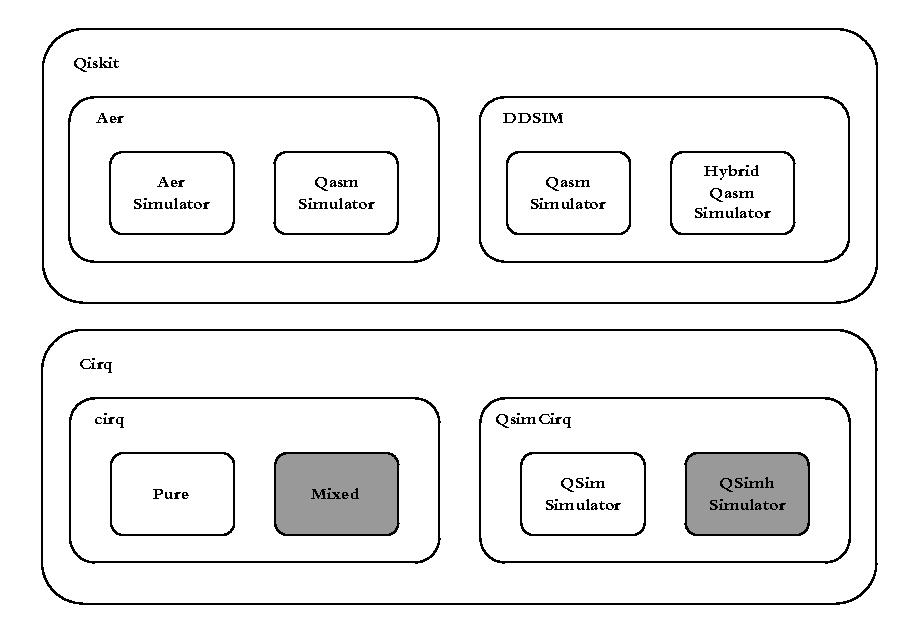
\includegraphics[scale=1]{images/backend_simulator_relation.pdf}
 	\caption{
 	نمودار روابط پلتفرم‌ها و اجزای آن‌ها (قسمت‌های خاکستری در پژوهش ما مورد بحث و بررسی نبوده‌اند.)
 	}
 	\label{fig:2}
 \end{figure}
 
\subsection{Qiskit}
 این پلتفرم توسط گروه تحقیقاتی IBM 
 \cite{javadi-abhari_quantum_2024}
 معرفی شده است که شامل چندین شبیه‌ساز با رویکردهای متفاوت شامل آن‌چه که در بخش
 \nameref{sec:simulators}
 گفته شده است. این پلتفرم علاوه بر شبیه‌ساز قابلیت‌هایی نظیر بهینه‌سازی و ترجمهٔ الگوریتم‌ها به زبان اسمبلی کوانتومی را نیز دارا است. علاوه‌برآن قابلیت اتصال به رایانه‌های واقعی کوانتومی ابری را نیز فراهم کرده است.
 
 هر پلتفرم برای جداسازی شبیه‌سازها باتوجه‌به رویکرد آن‌ها از بک‌اندهای متفاوت که همان لایه‌ای نرم‌افزاری باهدف چارچوب‌بندی به هر رویکرد شبیه‌سازی هستند، تشکیل شده است. در ادامه، شبیه‌سازها را به تفکیک بک‌اند، بررسی خواهیم کرد.
 
\subsubsection{Aer}
این بک‌اند شامل چهار شبیه‌ساز
\lr{AerSimulator}، \lr{QasmSimulator}، \lr{StatevectorSimulator} و \lr{UnitarySimulator}
است
\cite{javadi-abhari_quantum_2024}.
در پژوهش ما فقط به بررسی دو مورد اول پرداخته شده است.

\paragraph{:AerSimulator}
این شبیه‌ساز از چندین روش شبیه‌سازی و گزینه‌های قابل‌تنظیم برای هر روش شبیه‌سازی پشتیبانی می‌کند
\cite{noauthor_aersimulator_nodate}.
در محک این شبیه‌ساز، ابتدا الگوریتم‌های توضیح داده شده در بخش
\nameref{sec:algorithm_selection}
را اجرا و زمان اجرا و میزان حافظهٔ مصرفی آن را به تحریر نمودار درآورده‌ایم. نتیجهٔ حاصل شده در شکل‌های \ref{fig:3} و \ref{fig:4} نشانگر رفتار این شبیه‌ساز در اجرای الگوریتم‌های مختلف است.

از آن‌جایی که نتایج مربوط به الگوریتم Shor رفتار متفاوتی نسبت به دیگر الگوریتم‌ها داشته است، خروجی‌های مربوط به این الگوریتم در قالب جدول گزارش خواهد شد. این تفاوت در آن‌جایی است که برخلاف دیگر الگوریتم‌ها، داده‌های ورودی این الگوریتم محدودتر هستند و افزایش تعداد کیوبیت‌ها با افزایش عدد مرکب از دو عدد اول صورت می‌پذیرد. برای مثال در جدول \ref{tab:1} برای تجزیه‌ی عدد مرکب ۷۷ که از حاصل ضرب اعداد اول ۷ و ۱۱ بدست ‌می‌آید، الگوریتم Shor به ۲۴ کیوبیت احتیاج دارد تا بتواند این عدد را به عوامل اول آن تجزیه کند. به دلیل هم‌پوشانی که بین فاکتور‌های اول اعداد مرکب وجود دارد، نمی‌توان تعداد کیوبیت‌ها را یکی‌یکی افزایش داد و به همین دلیل زمان اجرا و حافظه‌ی مصرفی در قالب جداول نظیر جدول \ref{tab:1} گزارش شده است.

\begin{table}[h!]
	\centering
	\begin{LTR}
	\begin{tabular}{ |c|c|c|c| } 
		\hline
		\rl{عدد مرکب} & \rl{تعداد کیوبیت} & \rl{میانگین زمان اجرا (ثانیه)}  & \rl{میانگین حافظهٔ مصرفی (مگابایت)} \\
		\hline
		15 & 15 & 1.633536 & 121.723568 \\
		35 & 21 & 2.037188 & 122.529990 \\
		77 & 24 & 2.056493 & 125.207344 \\
		143 & 27 & 13.982873 & 129.990885 \\
		437 & 30 & N/A & N/A \\
		\hline
	\end{tabular}
	\end{LTR}
	\caption{
		جدول اطلاعات مربوط به اجرای الگوریتم Shor با
		\lr{Aer Simulator}
	}
	\label{tab:1}
\end{table}


\begin{figure}
	\centering
	\captionsetup{justification=centering}
	% This file was created with tikzplotlib v0.10.1.
\begin{tikzpicture}

	\definecolor{chocolate2267451}{RGB}{226,74,51}
	\definecolor{dimgray85}{RGB}{85,85,85}
	\definecolor{gainsboro229}{RGB}{229,229,229}
	\definecolor{gray119}{RGB}{119,119,119}
	\definecolor{lightgray204}{RGB}{204,204,204}
	\definecolor{mediumpurple152142213}{RGB}{152,142,213}
	\definecolor{sandybrown25119394}{RGB}{251,193,94}
	\definecolor{steelblue52138189}{RGB}{52,138,189}
	\definecolor{yellowgreen14218666}{RGB}{142,186,66}

	\begin{axis}[
    axis line style={black},
    tick style={black},
    grid=major,
    legend cell align={left},
    legend style={
        fill opacity=0.6,
        draw opacity=1,
        text opacity=1,
        at={(0.03,0.97)},
        anchor=north west,
        draw=lightgray204,
        fill=gainsboro229,
        font=\tiny,
        scale=0.1,
      },
    log basis y={10},
    tick align=outside,
    tick pos=left,
    x grid style={white},
    xlabel={\scriptsize\textcolor{black}{\rl{کیوبیت (عدد)}}},
    xmajorgrids,
    xmin=1, xmax=30,
    xtick distance=3,
    width=15cm,
    height=8cm,
    xtick style={color=dimgray85},
    y grid style={gray119},
    ylabel={\scriptsize\textcolor{black}{\rl{زمان اجرا (ثانیه)}}},
    ymajorgrids,
    ymin=0, ymax=3601,
    ymode=log,
    ytick style={color=dimgray85},
    ytick={1,10,100,1000,3600},
    yticklabels={
        \(\displaystyle {10^{0}}\),
        \(\displaystyle {10^{1}}\),
        \(\displaystyle {10^{2}}\),
        \(\displaystyle {10^{3}}\),
        \(\displaystyle {3600}\),
      },
    tick label style={font=\scriptsize}
  ]
		\addplot [semithick, chocolate2267451, dash pattern=on 1.5pt off 2.475pt, mark=*, mark size=3, mark options={solid}]
		table {%
				2 0.627046145969161
				3 0.620540094506347
				4 0.604433557288256
				5 0.557307506547704
				6 0.577668575013759
				7 0.619654589014544
				8 0.71398631361289
				9 0.808573271710126
				10 1.02579359791882
				11 1.70755112289388
				12 3.20736784415347
				13 7.18819421658966
				14 14.2466933424648
				15 35.4949261428393
				16 102.47516968324
				17 339.962429052473
				18 1280.15143594984
			};
		\addlegendentry{Deutsch-Jozsa (balanced)}
		\addplot [semithick, steelblue52138189, dash pattern=on 1.5pt off 2.475pt, mark=*, mark size=3, mark options={solid}]
		table {%
				2 0.619007757624548
				3 0.604727682732979
				4 0.599561547636613
				5 0.620342737456328
				6 0.58853850795581
				7 0.572819177000034
				8 0.603052117058198
				9 0.619279595640016
				10 0.576933875093806
				11 0.577723705664701
				12 0.600205244870589
				13 0.58294147643418
				14 0.553922971416598
				15 0.592418443107389
				16 0.610778429608383
				17 0.600022830768853
				18 0.590422668922574
				19 0.611738334022589
				20 0.654300124352312
				21 0.630325974868227
				22 0.63622559957729
				23 0.638434636725983
				24 0.597790644390853
				25 0.627876222588455
				26 0.608531387119575
				27 0.6158504437721
				28 0.617099424971479
			};
		\addlegendentry{Deutsch-Jozsa (constant)}
		\addplot [semithick, mediumpurple152142213, dash pattern=on 1.5pt off 2.475pt, mark=*, mark size=3, mark options={solid}]
		table {%
				2 0.625775995563965
				3 0.57775325457468
				4 0.600266677725543
				5 0.589891799900595
				6 0.587088828300655
				7 0.626464263387837
				8 0.583514458784009
				9 0.584047388728806
				10 0.622263500128114
				11 0.615194036042763
				12 0.598030297205431
				13 0.594709666634338
				14 0.627690367164237
				15 0.616887749775001
				16 0.595691669590584
				17 0.57740266146811
				18 0.571492576708758
				19 0.603566081606782
				20 0.606917118809959
				21 0.60262377817992
				22 0.593343016478124
				23 0.616170057293024
				24 0.61556207355751
				25 0.598909488495143
				26 0.597822427565701
				27 0.605887547693887
				28 0.627075332759571
			};
		\addlegendentry{Bernstein-Vazirani (basic)}
		\addplot [semithick, gray119, dash pattern=on 1.5pt off 2.475pt, mark=*, mark size=3, mark options={solid}]
		table {%
				2 0.573658010108471
				3 0.620933852126779
				4 0.565356786616637
				5 0.60226591831512
				6 0.603394420187709
				7 0.627239004985465
				8 0.622653529568651
				9 0.540358967517203
				10 0.577896496076911
				11 0.614049712703624
				12 0.578738785498038
				13 0.624202467350844
				14 0.607474514007616
				15 0.579391601718378
				16 0.583242387772462
				17 0.629852559202713
				18 0.70479680723381
				19 0.797260252629714
				20 0.900298026032862
				21 1.31753394724298
				22 2.10787159741243
				23 3.88590284328078
				24 7.52428175458831
				25 15.4287139293394
				26 31.9571831977387
				27 67.3291925381347
				28 142.335639079367
			};
		\addlegendentry{Quantum Fourier Transform (basic)}
		\addplot [semithick, sandybrown25119394, dash pattern=on 1.5pt off 2.475pt, mark=*, mark size=3, mark options={solid}]
		table {%
				2 2.20512034514554
				3 2.25890372158298
				4 2.20817412999522
				5 2.25658044806897
				6 2.23749479040781
				7 2.28594653873141
				8 2.29231295534857
				9 2.29971426264441
				10 2.263239687925
				11 2.30998097014085
				12 2.27261311829192
				13 2.26753437707271
				14 2.28446790319099
			};
		\addlegendentry{Simon (basic)}
		\addplot [semithick, yellowgreen14218666, dash pattern=on 1.5pt off 2.475pt, mark=*, mark size=3, mark options={solid}]
		table {%
				2 0.602772374542896
				3 0.635032709975031
				4 0.608714634228741
				5 0.606900246269116
				6 0.581898946577654
				7 0.589076310717568
				8 0.604531536341743
				9 0.612681784466321
				10 0.587272949534224
				11 0.604719892836494
				12 0.616668605208489
				13 0.556639777983306
				14 0.581914666579666
				15 0.598699448069502
				16 0.59577972315292
				17 0.615929523813299
				18 0.581640681853499
				19 0.676672037279193
				20 0.701376758362955
				21 0.844541243765989
				22 0.929530567222954
				23 1.2050532426835
				24 1.74018512284127
				25 3.02087841420321
				26 5.21255066366369
				27 10.796148155328
			};
		\addlegendentry{Grover (basic)}
	\end{axis}
\end{tikzpicture}

	\caption{
		نمودار زمان اجرا بر حسب تعداد کیوبیت الگوریتم‌های مختلف در
		\lr{Aer Simulator}
		}
	\label{fig:3}
	\vspace{2cm}
	\captionsetup{justification=centering}
	% This file was created with tikzplotlib v0.10.1.
\begin{tikzpicture}

	\definecolor{chocolate2267451}{RGB}{226,74,51}
	\definecolor{dimgray85}{RGB}{85,85,85}
	\definecolor{gainsboro229}{RGB}{229,229,229}
	\definecolor{gray119}{RGB}{119,119,119}
	\definecolor{lightgray204}{RGB}{204,204,204}
	\definecolor{mediumpurple152142213}{RGB}{152,142,213}
	\definecolor{sandybrown25119394}{RGB}{251,193,94}
	\definecolor{steelblue52138189}{RGB}{52,138,189}
	\definecolor{yellowgreen14218666}{RGB}{142,186,66}

	\begin{axis}[
		axis line style={black},  
		tick style={black},  
		grid=major,  
		legend cell align={left},
		legend style={
				fill opacity=0.6,
				draw opacity=1,
				text opacity=1,
				at={(0.03,0.97)},
				anchor=north west,  
				draw=lightgray204,
				fill=gainsboro229,
				font=\tiny,
				scale=0.1,
			},
		log basis y={10},
		tick align=outside,
		tick pos=left,
		x grid style={white},
		xlabel={\scriptsize\textcolor{black}{\rl{کیوبیت (عدد)}}},  
		xmajorgrids,
		xmin=1, xmax=30,
		xtick distance=3,
		width=15cm,
		height=8cm,
		xtick style={color=dimgray85, },
		y grid style={gray119},
		ylabel={\scriptsize\textcolor{black}{\rl{مصرف حافظه (مگابایت)}}},  
		ymajorgrids,
		ymin=0, ymax=16385,
		ymode=log,
		ytick style={color=dimgray85},
		ytick={512,1024,10240,16384},
		yticklabels={
				\(\displaystyle {512}\),
				\(\displaystyle {1024}\),
				\(\displaystyle {10240}\),
				\(\displaystyle {16384}\),
			},
		tick label style={font=\scriptsize}
	]
		\addplot [semithick, chocolate2267451, dash pattern=on 1.5pt off 2.475pt, mark=*, mark size=3, mark options={solid}]
		table {%
				2 87.4186197916667
				3 87.44921875
				4 87.5455729166667
				5 87.8248697916667
				6 88.408203125
				7 88.4466145833333
				8 89.8626302083333
				9 92.5182291666667
				10 99.9869791666667
				11 116.418619791667
				12 148.608072916667
				13 219.912109375
				14 374.431640625
				15 696.547526041667
				16 1376.69661458333
				17 2812.40299479167
				18 5715.953125
			};
		\addlegendentry{Deutsch-Jozsa (balanced)}
		\addplot [semithick, steelblue52138189, dash pattern=on 1.5pt off 2.475pt, mark=*, mark size=3, mark options={solid}]
		table {%
				2 87.475
				3 87.175
				4 87.3484375
				5 87.38828125
				6 87.4828125
				7 87.121875
				8 87.43359375
				9 87.44140625
				10 87.5109375
				11 87.359375
				12 87.59609375
				13 87.4703125
				14 87.50546875
				15 87.428125
				16 87.50625
				17 87.2453125
				18 87.4296875
				19 87.6078125
				20 87.42265625
				21 87.6171875
				22 87.4046875
				23 87.29375
				24 87.76015625
				25 87.28125
				26 87.69765625
				27 87.740625
				28 87.54921875
			};
		\addlegendentry{Deutsch-Jozsa (constant)}
		\addplot [semithick, mediumpurple152142213, dash pattern=on 1.5pt off 2.475pt, mark=*, mark size=3, mark options={solid}]
		table {%
				2 87.2953125
				3 87.3328125
				4 87.55078125
				5 87.40078125
				6 87.10390625
				7 87.36875
				8 87.421875
				9 87.4109375
				10 87.20625
				11 87.48046875
				12 87.309375
				13 87.39609375
				14 87.10859375
				15 87.5421875
				16 87.3953125
				17 87.6125
				18 87.6265625
				19 87.70234375
				20 87.83359375
				21 88.01640625
				22 87.99140625
				23 88.0875
				24 88.040625
				25 87.72578125
				26 87.9578125
				27 87.96328125
				28 88.15625
			};
		\addlegendentry{Bernstein-Vazirani (basic)}
		\addplot [semithick, gray119, dash pattern=on 1.5pt off 2.475pt, mark=*, mark size=3, mark options={solid}]
		table {%
				2 86.9890625
				3 87.16640625
				4 87.26953125
				5 87.2453125
				6 87.54375
				7 87.415625
				8 87.484375
				9 87.85546875
				10 87.821875
				11 88.05078125
				12 88.1421875
				13 88.146875
				14 88.34453125
				15 88.67578125
				16 88.19921875
				17 88.58828125
				18 90.43203125
				19 94.90390625
				20 103.42109375
				21 119.759375
				22 152.7625
				23 216.6640625
				24 345.0125
				25 600.96171875
				26 1113.103125
				27 2136.6515625
				28 4184.44765625
			};
		\addlegendentry{Quantum Fourier Transform (basic)}
		\addplot [semithick, sandybrown25119394, dash pattern=on 1.5pt off 2.475pt, mark=*, mark size=3, mark options={solid}]
		table {%
				2 229.48359375
				3 229.76328125
				4 229.2375
				5 229.5859375
				6 229.3890625
				7 229.5078125
				8 229.37421875
				9 229.82578125
				10 230.20078125
				11 230.0484375
				12 229.82890625
				13 229.86953125
				14 230.175
			};
		\addlegendentry{Simon (basic)}
		\addplot [semithick, yellowgreen14218666, dash pattern=on 1.5pt off 2.475pt, mark=*, mark size=3, mark options={solid}]
		table {%
				2 87.5729166666667
				3 87.85546875
				4 87.86171875
				5 88.015625
				6 87.98671875
				7 87.853125
				8 87.88203125
				9 88.59921875
				10 88.46796875
				11 88.5484375
				12 88.64453125
				13 88.8578125
				14 89.4328125
				15 88.73203125
				16 88.7625
				17 88.6421875
				18 88.7015625
				19 102.64921875
				20 119.21484375
				21 151.7375
				22 215.79609375
				23 343.65859375
				24 599.646875
				25 1111.14453125
				26 2134.63359375
				27 4182.31484375
			};
		\addlegendentry{Grover (basic)}
	\end{axis}
\end{tikzpicture}

	\caption{
		نمودار مصرف حافظه بر حسب تعداد کیوبیت الگوریتم‌های مختلف
		\lr{Aer Simulator}
		}
	\label{fig:4}
\end{figure}

 از آن‌جایی که در محدودیت‌های این شبیه‌ساز تعداد ۳۲ کیوبیت ذکر شده همان‌طور که مشاهده می‌شود این شبیه‌ساز، در این محدوده، در اجرای همهٔ الگوریتم‌ها همان‌طور که انتظار می‌رود رفتار کرده است. دلیل این که محک با الگوریتمی نظیر Simon فقط تا ۱۶ کیوبیت ادامه پیدا کرده است این است که این الگوریتم برای حل مسئله به دوبرابر تعداد کیوبیت ورودی نیاز دارد. دیگر الگوریتم‌ها نظیر
 \lr{Grover}
 در تعداد کیوبیت کمتر رفتاری خطی و با افزایش تعداد کیوبیت رفتاری نمایی به خود می‌گیرند، طبق آن‌چه که در 
 \cite{jamadagni_benchmarking_2024}
 هم حدس زده شده است، امکان بهینه‌سازی غیر جامع این شبیه‌سازها به‌طوری‌که برای تعداد کیوبیت کمتر، بهینه شده باشند، وجود دارد.
  
  
\paragraph{:QasmSimulator}
این شبیه‌ساز هم از چندین روش شبیه‌سازی و اضافه‌کردن نویز به محاسبات پشتیبانی می‌کند. مانند قبل، اجرای الگوریتم‌ها با این شبیه‌ساز، در شکل‌ \ref{fig:5} برای زمان اجرا و در شکل \ref{fig:6} برای مصرف حافظه، آورده شده است.

\begin{figure}
	\centering
	\captionsetup{justification=centering}
	% This file was created with tikzplotlib v0.10.1.
\begin{tikzpicture}

	\definecolor{chocolate2267451}{RGB}{226,74,51}
	\definecolor{dimgray85}{RGB}{85,85,85}
	\definecolor{gainsboro229}{RGB}{229,229,229}
	\definecolor{gray119}{RGB}{119,119,119}
	\definecolor{lightgray204}{RGB}{204,204,204}
	\definecolor{mediumpurple152142213}{RGB}{152,142,213}
	\definecolor{sandybrown25119394}{RGB}{251,193,94}
	\definecolor{steelblue52138189}{RGB}{52,138,189}
	\definecolor{yellowgreen14218666}{RGB}{142,186,66}

	\begin{axis}[
    axis line style={black},
    tick style={black},
    grid=major,
    legend cell align={left},
    legend style={
        fill opacity=0.6,
        draw opacity=1,
        text opacity=1,
        at={(0.03,0.97)},
            anchor=north west,
        draw=lightgray204,
        fill=gainsboro229,
        font=\tiny,
        scale=0.1,
      },
    log basis y={10},
    tick align=outside,
    tick pos=left,
    x grid style={white},
    xlabel={\scriptsize\textcolor{black}{\rl{کیوبیت (عدد)}}},
    xmajorgrids,
    xmin=1, xmax=30,
    xtick distance=3,
    width=15cm,
    height=8cm,
    xtick style={color=dimgray85},
    y grid style={gray119},
    ylabel={\scriptsize\textcolor{black}{\rl{زمان اجرا (ثانیه)}}},
    ymajorgrids,
    ymin=0, ymax=3601,
    ymode=log,
    ytick style={color=dimgray85},
    ytick={1,10,100,1000,3600},
    yticklabels={
        \(\displaystyle {10^{0}}\),
        \(\displaystyle {10^{1}}\),
        \(\displaystyle {10^{2}}\),
        \(\displaystyle {10^{3}}\),
        \(\displaystyle {3600}\),
      },
    tick label style={font=\scriptsize}
  ]
		\addplot [semithick, chocolate2267451, dash pattern=on 1.5pt off 2.475pt, mark=*, mark size=3, mark options={solid}]
		table {%
				2 0.591304939326721
				3 0.618261231849203
				4 0.577479210922229
				5 0.628029825778719
				6 0.585005118487057
				7 0.599685080375904
				8 0.686506206148601
				9 0.757161041830157
				10 1.10488201718041
				11 1.75085018115432
				12 3.20639903344505
				13 7.15465083628399
				14 14.1702002220477
				15 35.5978986419106
				16 101.968037412245
				17 335.167788917545
				18 1284.39366972227
			};
		\addlegendentry{Deutsch-Jozsa (balanced)}
		\addplot [semithick, steelblue52138189, dash pattern=on 1.5pt off 2.475pt, mark=*, mark size=3, mark options={solid}]
		table {%
				2 0.551828144253206
				3 0.590439638488487
				4 0.567508328243958
				5 0.59823508426399
				6 0.621217404316689
				7 0.59946020230677
				8 0.586307117425776
				9 0.586612219671519
				10 0.607149356791602
				11 0.615608784099126
				12 0.587470683262726
				13 0.597111710344613
				14 0.632774829102299
				15 0.60417722842819
				16 0.598305650532505
				17 0.607249654493505
				18 0.596454103639309
				19 0.648430512579695
				20 0.610270239995572
				21 0.592256275573141
				22 0.591027687882309
				23 0.589262959065021
				24 0.601417301357851
				25 0.608057674837554
				26 0.594927006095338
				27 0.594472514747671
				28 0.612312020066186
			};
		\addlegendentry{Deutsch-Jozsa (constant)}
		\addplot [semithick, mediumpurple152142213, dash pattern=on 1.5pt off 2.475pt, mark=*, mark size=3, mark options={solid}]
		table {%
				2 0.629261635662515
				3 0.609867073800108
				4 0.572150678443529
				5 0.587133596952081
				6 0.604671435789041
				7 0.584635582594932
				8 0.622253316099649
				9 0.643627386165328
				10 0.634817802946494
				11 0.631513573105945
				12 0.581876545091362
				13 0.600967388597273
				14 0.633275790308154
				15 0.610229784309262
				16 0.617165758490921
				17 0.59918137634296
				18 0.575291403778686
				19 0.586644503646457
				20 0.592540540725066
				21 0.570599611521831
				22 0.609072857566842
				23 0.61669186193905
				24 0.610933927341243
				25 0.558536567458387
				26 0.579453378659335
				27 0.64195073023149
				28 0.607336142368001
			};
		\addlegendentry{Bernstein-Vazirani (basic)}
		\addplot [semithick, gray119, dash pattern=on 1.5pt off 2.475pt, mark=*, mark size=3, mark options={solid}]
		table {%
				2 0.563773031268817
				3 0.606310363437206
				4 0.626277882479424
				5 0.576788003446191
				6 0.582043068814394
				7 0.584138188967175
				8 0.556127427303879
				9 0.600190367513802
				10 0.61637415972298
				11 0.567178715037237
				12 0.609194127338951
				13 0.599344623938434
				14 0.605959790438121
				15 0.602827551586954
				16 0.597538671964051
				17 0.615186895679008
				18 0.686632744027427
				19 0.823638496072659
				20 0.98668141403423
				21 1.32044579789538
				22 2.15365708599401
				23 3.83974180395365
				24 7.56726772410653
				25 15.3069594878619
				26 32.1641921493779
				27 66.6852066668747
				28 142.767433474461
			};
		\addlegendentry{Quantum Fourier Transform (basic)}
		\addplot [semithick, sandybrown25119394, dash pattern=on 1.5pt off 2.475pt, mark=*, mark size=3, mark options={solid}]
		table {%
				2 2.25752379481232
				3 2.22970408734623
				4 2.22059319063216
				5 2.29589687441571
				6 2.24933181212165
				7 2.25391943622014
				8 2.28917567009626
				9 2.24331593991242
				10 2.25624203202973
				11 2.30272481055481
				12 2.30446695755306
				13 2.2845832516284
				14 2.31855734806885
			};
		\addlegendentry{Simon (basic)}
		\addplot [semithick, yellowgreen14218666, dash pattern=on 1.5pt off 2.475pt, mark=*, mark size=3, mark options={solid}]
		table {%
				2 0.649931628978543
				3 0.602191712238641
				4 0.579303999019014
				5 0.569967556803601
				6 0.608636965171304
				7 0.602942172379934
				8 0.628092795066265
				9 0.618951065669277
				10 0.593648011805128
				11 0.586805968356733
				12 0.626033275122053
				13 0.582294830908879
				14 0.596098828523707
				15 0.63659568658484
				16 0.632872437906449
				17 0.619900140388033
				18 0.580904288024011
				19 0.601640522692469
				20 0.67308033251598
				21 0.813011315558499
				22 0.901670418415067
				23 1.19198870973306
				24 1.69104096492784
				25 3.01485940653384
				26 5.22743925279817
				27 10.8084091084026
			};
		\addlegendentry{Grover (basic)}
	\end{axis}
\end{tikzpicture}

	\caption{
		نمودار زمان اجرا بر حسب تعداد کیوبیت الگوریتم‌های مختلف در 
		\lr{Qasm Simulator}
		}
	\label{fig:5}
	\vspace{2cm}
	\captionsetup{justification=centering}
	% This file was created with tikzplotlib v0.10.1.
\begin{tikzpicture}

	\definecolor{chocolate2267451}{RGB}{226,74,51}
	\definecolor{dimgray85}{RGB}{85,85,85}
	\definecolor{gainsboro229}{RGB}{229,229,229}
	\definecolor{gray119}{RGB}{119,119,119}
	\definecolor{lightgray204}{RGB}{204,204,204}
	\definecolor{mediumpurple152142213}{RGB}{152,142,213}
	\definecolor{sandybrown25119394}{RGB}{251,193,94}
	\definecolor{steelblue52138189}{RGB}{52,138,189}
	\definecolor{yellowgreen14218666}{RGB}{142,186,66}

	\begin{axis}[
		axis line style={black},  
		tick style={black},  
		grid=major,  
		legend cell align={left},
		legend style={
				fill opacity=0.6,
				draw opacity=1,
				text opacity=1,
				at={(0.03,0.97)},
				anchor=north west,  
				draw=lightgray204,
				fill=gainsboro229,
				font=\tiny,
				scale=0.1,
			},
		log basis y={10},
		tick align=outside,
		tick pos=left,
		x grid style={white},
		xlabel={\scriptsize\textcolor{black}{\rl{کیوبیت (عدد)}}},  
		xmajorgrids,
		xmin=1, xmax=30,
		xtick distance=3,
		width=15cm,
		height=8cm,
		xtick style={color=dimgray85, },
		y grid style={gray119},
		ylabel={\scriptsize\textcolor{black}{\rl{مصرف حافظه (مگابایت)}}},  
		ymajorgrids,
		ymin=0, ymax=16385,
		ymode=log,
		ytick style={color=dimgray85},
		ytick={512,1024,10240,16384},
		yticklabels={
				\(\displaystyle {512}\),
				\(\displaystyle {1024}\),
				\(\displaystyle {10240}\),
				\(\displaystyle {16384}\),
			},
		tick label style={font=\scriptsize}
	]
		\addplot [semithick, chocolate2267451, dash pattern=on 1.5pt off 2.475pt, mark=*, mark size=3, mark options={solid}]
		table {%
				2 87.5735677083333
				3 87.5924479166667
				4 87.6360677083333
				5 87.8001302083333
				6 88.2115885416667
				7 87.9498697916667
				8 89.7740885416667
				9 92.689453125
				10 99.71875
				11 116.413411458333
				12 148.22265625
				13 220.29296875
				14 378.317057291667
				15 691.319661458333
				16 1394.033203125
				17 2812.29557291667
				18 5734.58658854167
			};
		\addlegendentry{Deutsch-Jozsa (balanced)}
		\addplot [semithick, steelblue52138189, dash pattern=on 1.5pt off 2.475pt, mark=*, mark size=3, mark options={solid}]
		table {%
				2 87.19296875
				3 87.17265625
				4 87.303125
				5 87.41015625
				6 87.3859375
				7 87.459375
				8 87.3203125
				9 87.325
				10 87.23515625
				11 87.271875
				12 87.35078125
				13 87.3453125
				14 87.47265625
				15 87.31171875
				16 87.61484375
				17 87.3671875
				18 87.428125
				19 87.44921875
				20 87.709375
				21 87.45703125
				22 87.3140625
				23 87.4671875
				24 87.509375
				25 87.465625
				26 87.515625
				27 87.85078125
				28 87.7203125
			};
		\addlegendentry{Deutsch-Jozsa (constant)}
		\addplot [semithick, mediumpurple152142213, dash pattern=on 1.5pt off 2.475pt, mark=*, mark size=3, mark options={solid}]
		table {%
				2 87.2375
				3 87.02421875
				4 87.428125
				5 87.09453125
				6 87.3265625
				7 87.51328125
				8 87.28828125
				9 87.31484375
				10 87.47421875
				11 87.42734375
				12 87.478125
				13 87.19921875
				14 87.37265625
				15 87.8515625
				16 87.79375
				17 87.99140625
				18 87.7203125
				19 87.69296875
				20 87.7203125
				21 87.90859375
				22 88.07109375
				23 88.19609375
				24 88.13125
				25 88.20546875
				26 88.21171875
				27 88.0859375
				28 88.05078125
			};
		\addlegendentry{Bernstein-Vazirani (basic)}
		\addplot [semithick, gray119, dash pattern=on 1.5pt off 2.475pt, mark=*, mark size=3, mark options={solid}]
		table {%
				2 87.19375
				3 87.2796875
				4 87.21328125
				5 87.1296875
				6 87.484375
				7 87.4578125
				8 87.4359375
				9 87.871875
				10 88.00390625
				11 88.0015625
				12 88.09609375
				13 88.046875
				14 88.259375
				15 88.9859375
				16 88.07578125
				17 88.89140625
				18 88.85390625
				19 95.175
				20 103.3015625
				21 119.79609375
				22 152.88671875
				23 216.72890625
				24 345.0578125
				25 601.03203125
				26 1113.0140625
				27 2136.5984375
				28 4184.321875
			};
		\addlegendentry{Quantum Fourier Transform (basic)}
		\addplot [semithick, sandybrown25119394, dash pattern=on 1.5pt off 2.475pt, mark=*, mark size=3, mark options={solid}]
		table {%
				2 229.528125
				3 229.52578125
				4 229.37421875
				5 229.559375
				6 229.3640625
				7 229.47734375
				8 229.240625
				9 229.7171875
				10 229.85
				11 230.0359375
				12 230.13046875
				13 230.240625
				14 230.0828125
			};
		\addlegendentry{Simon (basic)}
		\addplot [semithick, yellowgreen14218666, dash pattern=on 1.5pt off 2.475pt, mark=*, mark size=3, mark options={solid}]
		table {%
				2 87.8736979166667
				3 87.93671875
				4 87.99296875
				5 88.325
				6 88.15703125
				7 88.21953125
				8 88.51015625
				9 88.32578125
				10 88.53671875
				11 88.53515625
				12 88.496875
				13 88.63046875
				14 89.03515625
				15 88.8109375
				16 88.92265625
				17 88.7890625
				18 90.925
				19 102.79375
				20 119.16953125
				21 151.8796875
				22 215.65234375
				23 343.571875
				24 599.48515625
				25 1111.06328125
				26 2134.353125
				27 4182.3015625
			};
		\addlegendentry{Grover (basic)}
	\end{axis}
\end{tikzpicture}

	\caption{
		نمودار مصرف حافظه بر حسب تعداد کیوبیت الگوریتم‌های مختلف در
		\lr{Qasm Simulator}
		}
	\label{fig:6}
\end{figure}

از آن‌جایی که این دو شبیه‌ساز در یک بک‌اند توسعه داده شده‌اند، تفاوت چندانی در عملکرد آن‌ها مشاهده نمی‌شود و رفتار مشابهی را در مواجهه با الگوریتم‌های مختلف دارند که این رفتار موردانتظار از شبیه‌سازهای مدارهای کوانتومی است.

به صورت مجزا، عملکرد این شبیه‌ساز در اجرای الگوریتم Shor در جدول \ref{tab:2} گزارش شده است.
\begin{table}[h!]
	\centering
	\begin{LTR}
		\begin{tabular}{ |c|c|c|c| } 
			\hline
			\rl{عدد مرکب} & \rl{تعداد کیوبیت} & \rl{میانگین زمان اجرا (ثانیه)}  & \rl{میانگین حافظهٔ مصرفی (مگابایت)} \\
			\hline
			15 & 15 & 1.770852 & 121.732682 \\
			35 & 21 & 3.714265 & 123.226562 \\
			77 & 24 & 2.542166 & 125.411875 \\
			143 & 27 & 14.051529 & 130.393229 \\
			437 & 30 & N/A & N/A \\
			\hline
		\end{tabular}
	\end{LTR}
	\caption{
		جدول اطلاعات مربوط به اجرای الگوریتم Shor با
		\lr{Qasm Simulator}
	}
	\label{tab:2}
\end{table}
 
\subsubsection{DDSIM}
این بک‌اند چهارچوبی برای شبیه‌سازها تعیین کرده است که از یک روش مبتنی بر گراف، به‌ویژه نمودارهای تصمیم‌گیری، برای شبیه‌سازی کارآمد مدارهای کوانتومی استفاده می‌کند و به‌جای ذخیره بردارها و ماتریس‌های بزرگی که به‌صورت نمایی رشد می‌کنند، از این نمودارها برای ثبت تکرارهای موجود در محاسبات بهره می‌برد. در واقع به نحوی از برنامه‌نویسی پویا برای بهبود کارایی شبیه‌سازی استفاده می‌کند و به‌این‌ترتیب استفاده از حافظه را به میزان قابل‌توجهی کاهش می‌دهد. عملیات کوانتومی از طریق ضرب ماتریس‌ها و بردارها در این قالب به‌صورت بازگشتی انجام می‌شوند بدون این که نیاز باشد کل آن‌ها پردازش شوند. اندازه‌گیری نیز به همین شکل انجام می‌شود و تغییرات حالت به طور کارآمد در نمودارها نمایش داده می‌شود. این روش باعث می‌شود که این نوع از شبیه‌سازها در مقایسه با شبیه‌سازهای دیگر، عملکرد بهتری داشته باشند و بتوانند تعداد بیش‌تری کیوبیت را مدیریت کنند و زمان و حافظهٔ محاسباتی کمتری مصرف کنند 
\cite{zulehner_advanced_2019}.
\paragraph{:QasmSimulator}
این شبیه‌ساز از روش Schrödinger استفاده می‌کند که بر اساس نمودارهای تصمیم‌گیری به‌عنوان یک ساختمان داده، طراحی شده و می‌توان از آن برای به‌دست‌آوردن بردار حالت کامل مدار کوانتومی «شبیه‌سازی قوی» 
\cite{zulehner_advanced_2019}
و یا نمونه‌گیری از توزیع خروجی یک مدار کوانتومی «شبیه‌سازی ضعیف» 
\cite{hillmich_just_2020}
بهره برد. برای این منظور، شبیه‌ساز با نمایش نمودار تصمیم‌گیری از حالت اولیه آغاز می‌شود و سپس در هر مرحله، گیت‌های مدار را یکی‌یکی اعمال می‌کند. نمایش نمودار تصمیم‌گیری از بردار حالت در هر مرحله به‌روزرسانی می‌شود. این شبیه‌ساز قادر است مدارهای کوانتومی تقریباً دلخواه، از جمله مدارهایی با اندازه‌گیری‌ها و بازتنظیم‌های میانی را مدیریت کند. برای مدارهایی که شامل عملیات غیر واحدی (به‌جز اندازه‌گیری‌ها در انتهای مدار) نیستند، شبیه‌سازی فقط یک‌بار انجام می‌شود. در این حالت، تعداد نمونه‌های درخواستی به طور متعاقب از نمودار تصمیم‌گیری نهایی گرفته می‌شود که منجر به زمان اجرای سریع شبیه‌سازی می‌گردد.

شایان‌ذکر است که این شبیه‌ساز با شبیه‌سازی که در قسمت قبل توضیح داده شده است، متفاوت است. با این که هر دو از روش Schrödinger برای شبیه‌سازی بهره گرفته‌اند؛ اما ساختمان داده‌ای که در شبیه‌ساز دوم با بک‌اند DDSIM توسعه‌یافته به طور کامل با شبیه‌ساز با بک‌اند Aer متفاوت است.

\begin{figure}
	\centering
	\captionsetup{justification=centering}
	% This file was created with tikzplotlib v0.10.1.
\begin{tikzpicture}

	\definecolor{chocolate2267451}{RGB}{226,74,51}
	\definecolor{dimgray85}{RGB}{85,85,85}
	\definecolor{gainsboro229}{RGB}{229,229,229}
	\definecolor{gray119}{RGB}{119,119,119}
	\definecolor{lightgray204}{RGB}{204,204,204}
	\definecolor{mediumpurple152142213}{RGB}{152,142,213}
	\definecolor{sandybrown25119394}{RGB}{251,193,94}
	\definecolor{steelblue52138189}{RGB}{52,138,189}

	\begin{axis}[
    axis line style={black},
    tick style={black},
    grid=major,
    legend cell align={left},
    legend style={
        fill opacity=0.6,
        draw opacity=1,
        text opacity=1,
        at={(0.03,0.97)},
            anchor=north west,
        draw=lightgray204,
        fill=gainsboro229,
        font=\tiny,
        scale=0.1,
      },
    log basis y={10},
    tick align=outside,
    tick pos=left,
    x grid style={white},
    xlabel={\scriptsize\textcolor{black}{\rl{کیوبیت (عدد)}}},
    xmajorgrids,
    xmin=1, xmax=30,
    xtick distance=3,
    width=15cm,
    height=8cm,
    xtick style={color=dimgray85},
    y grid style={gray119},
    ylabel={\scriptsize\textcolor{black}{\rl{زمان اجرا (ثانیه)}}},
    ymajorgrids,
    ymin=0, ymax=3601,
    ymode=log,
    ytick style={color=dimgray85},
    ytick={1,10,100,1000,3600},
    yticklabels={
        \(\displaystyle {10^{0}}\),
        \(\displaystyle {10^{1}}\),
        \(\displaystyle {10^{2}}\),
        \(\displaystyle {10^{3}}\),
        \(\displaystyle {3600}\),
      },
    tick label style={font=\scriptsize}
  ]
		\addplot [semithick, chocolate2267451, dash pattern=on 1.5pt off 2.475pt, mark=*, mark size=3, mark options={solid}]
		table {%
				2 0.612252539865214
				3 0.601244009112429
				4 0.593100177356242
				5 0.599033548432153
				6 0.588201006522595
				7 0.696863817125534
				8 0.807233468592781
				9 1.13087342554267
				10 1.71884750350639
				11 3.10042611536326
				12 6.16515288339251
				13 13.8144959049632
				14 33.8972658858413
				15 92.8064641957886
				16 276.278772114309
				17 957.045420053034
			};
		\addlegendentry{Deutsch-Jozsa (balanced)}
		\addplot [semithick, steelblue52138189, dash pattern=on 1.5pt off 2.475pt, mark=*, mark size=3, mark options={solid}]
		table {%
				2 0.581679406032504
				3 0.583822387977432
				4 0.554115560236107
				5 0.604149132044441
				6 0.625254636644959
				7 0.620841372833219
				8 0.603722554715012
				9 0.621960763666647
				10 0.555654150495092
				11 0.616124791177196
				12 0.607931797965015
				13 0.597951840958091
				14 0.599682196553941
				15 0.592530303824046
				16 0.598625423020701
				17 0.593269360834072
				18 0.599336407179625
				19 0.587269851931074
				20 0.574376530453162
				21 0.620605356850644
				22 0.612003996071707
				23 0.614884185756279
				24 0.593040984237245
				25 0.585609606902293
				26 0.584196067951382
				27 0.593606885921734
				28 0.595821913605421
				29 0.62102413421069
			};
		\addlegendentry{Deutsch-Jozsa (constant)}
		\addplot [semithick, mediumpurple152142213, dash pattern=on 1.5pt off 2.475pt, mark=*, mark size=3, mark options={solid}]
		table {%
				2 0.587890294405024
				3 0.607217057347551
				4 0.594140859327094
				5 0.608088254226921
				6 0.570405318564412
				7 0.611789878501847
				8 0.625440780474689
				9 0.628608712815088
				10 0.594298879911107
				11 0.61193676720635
				12 0.569981662448604
				13 0.56787768890125
				14 0.596789004360342
				15 0.625093936909044
				16 0.580766247407487
				17 0.588977490424729
				18 0.599994484817433
				19 0.585004511304591
				20 0.621772335048289
				21 0.627481898696414
				22 0.617059661434273
				23 0.605341294828682
				24 0.601486240354653
				25 0.564193096421025
				26 0.595621089723595
				27 0.606451361787534
				28 0.606056650122247
				29 0.631891646089077
			};
		\addlegendentry{Bernstein-Vazirani (basic)}
		\addplot [semithick, gray119, dash pattern=on 1.5pt off 2.475pt, mark=*, mark size=3, mark options={solid}]
		table {%
				2 1.02784112379512
				3 0.610807095489116
				4 0.609624942989935
				5 0.593514286111592
				6 0.58695403577948
				7 0.589214627628456
				8 0.600340207582892
				9 0.616284045165562
				10 0.616076385429282
				11 0.603170323702486
				12 0.594240256305975
				13 0.626532288466614
				14 0.598152303267251
				15 0.6351940589673
				16 0.699118805171104
				17 0.720838692816472
				18 0.817515612120289
				19 0.9790566556133
				20 1.10810050962505
				21 1.78353961277023
				22 2.44386672673494
				23 4.62526021299006
				24 9.7430977261344
				25 18.1854031520582
				26 37.1694594946284
				27 64.7092330153807
				28 146.479316623025
				29 280.034649538871
			};
		\addlegendentry{Quantum Fourier Transform (basic)}
		\addplot [semithick, sandybrown25119394, dash pattern=on 1.5pt off 2.475pt, mark=*, mark size=3, mark options={solid}]
		table {%
				2 0.591846040119179
				3 0.630324380985934
				4 0.570937748298535
				5 0.596453599062918
				6 0.613574608037819
				7 0.596186930927414
				8 0.603409369202958
				9 0.652565426564348
				10 0.618473927028231
				11 0.575762926989485
				12 0.605624820432406
				13 0.626369027859028
				14 0.632398366185987
				15 0.632420712927039
				16 0.616576239492234
				17 0.633317724737592
				18 0.617690554121882
				19 0.631588403936496
				20 0.615689365074128
				21 0.631977333883819
				22 0.589721571302832
				23 0.592716939375255
				24 0.603072703158856
				25 0.592843291320397
				26 0.589109646095748
				27 0.646674980634838
				28 0.636228435303491
				29 0.57088168193142
			};
		\addlegendentry{Grover (basic)}
	\end{axis}
\end{tikzpicture}

	\caption{
		نمودار زمان اجرا بر حسب تعداد کیوبیت الگوریتم‌های مختلف در
		\lr{DDSIM Qasm Simulator}
		}
	\label{fig:7}
	\vspace{2cm}
	\captionsetup{justification=centering}
	% This file was created with tikzplotlib v0.10.1.
\begin{tikzpicture}

	\definecolor{chocolate2267451}{RGB}{226,74,51}
	\definecolor{dimgray85}{RGB}{85,85,85}
	\definecolor{gainsboro229}{RGB}{229,229,229}
	\definecolor{gray119}{RGB}{119,119,119}
	\definecolor{lightgray204}{RGB}{204,204,204}
	\definecolor{mediumpurple152142213}{RGB}{152,142,213}
	\definecolor{sandybrown25119394}{RGB}{251,193,94}
	\definecolor{steelblue52138189}{RGB}{52,138,189}

	\begin{axis}[
    axis line style={black},  
    tick style={black},  
    grid=major,  
    legend cell align={left},
    legend style={
        fill opacity=0.6,
        draw opacity=1,
        text opacity=1,
        at={(0.03,0.97)},
            anchor=north west,  
        draw=lightgray204,
        fill=gainsboro229,
        font=\tiny,
        scale=0.1,
      },
    log basis y={10},
    tick align=outside,
    tick pos=left,
    x grid style={white},
    xlabel={\scriptsize\textcolor{black}{\rl{کیوبیت (عدد)}}},  
    xmajorgrids,
    xmin=1, xmax=30,
    xtick distance=3,
    width=15cm,
    height=8cm,
    xtick style={color=dimgray85, },
    y grid style={gray119},
    ylabel={\scriptsize\textcolor{black}{\rl{مصرف حافظه (مگابایت)}}},  
    ymajorgrids,
    ymin=0, ymax=16385,
    ymode=log,
    ytick style={color=dimgray85},
    ytick={512,1024,10240,16384},
    yticklabels={
        \(\displaystyle {512}\),
        \(\displaystyle {1024}\),
        \(\displaystyle {10240}\),
        \(\displaystyle {16384}\),
      },
    tick label style={font=\scriptsize}
  ]
		\addplot [semithick, chocolate2267451, dash pattern=on 1.5pt off 2.475pt, mark=*, mark size=3, mark options={solid}]
		table {%
				2 87.8625
				3 87.86796875
				4 87.8390625
				5 87.95234375
				6 97.40234375
				7 89.33828125
				8 90.4515625
				9 91.82734375
				10 99.365625
				11 136.46328125
				12 152.90703125
				13 179.47734375
				14 231.49375
				15 345.29375
				16 617.43828125
				17 1206.96875
			};
		\addlegendentry{Deutsch-Jozsa (balanced)}
		\addplot [semithick, steelblue52138189, dash pattern=on 1.5pt off 2.475pt, mark=*, mark size=3, mark options={solid}]
		table {%
				2 87.95703125
				3 87.70390625
				4 87.85390625
				5 87.9203125
				6 87.86640625
				7 87.6640625
				8 87.7734375
				9 88.0140625
				10 87.88046875
				11 87.8296875
				12 87.9625
				13 87.78671875
				14 88.1328125
				15 87.8359375
				16 87.809375
				17 87.82890625
				18 88.0640625
				19 87.96875
				20 87.96796875
				21 87.83671875
				22 88.2640625
				23 88.07890625
				24 88.2703125
				25 88.33515625
				26 88.24375
				27 88.396875
				28 88.4890625
				29 88.5140625
			};
		\addlegendentry{Deutsch-Jozsa (constant)}
		\addplot [semithick, mediumpurple152142213, dash pattern=on 1.5pt off 2.475pt, mark=*, mark size=3, mark options={solid}]
		table {%
				2 87.9140625
				3 87.8359375
				4 87.79296875
				5 87.75078125
				6 88.0078125
				7 87.8359375
				8 87.7359375
				9 88.16640625
				10 87.846875
				11 87.9
				12 87.76484375
				13 87.6921875
				14 88.37578125
				15 87.90546875
				16 88.31484375
				17 88.121875
				18 88.61484375
				19 88.55625
				20 88.121875
				21 88.53046875
				22 88.225
				23 88.41328125
				24 88.34453125
				25 88.4953125
				26 88.54140625
				27 88.3859375
				28 88.128125
				29 88.51484375
			};
		\addlegendentry{Bernstein-Vazirani (basic)}
		\addplot [semithick, gray119, dash pattern=on 1.5pt off 2.475pt, mark=*, mark size=3, mark options={solid}]
		table {%
				2 87.4109375
				3 87.709375
				4 87.65078125
				5 87.6453125
				6 87.6484375
				7 87.9546875
				8 87.60234375
				9 88.16875
				10 87.87890625
				11 88.221875
				12 88.084375
				13 90.8375
				14 110.4453125
				15 105.90078125
				16 110.46171875
				17 105.2296875
				18 110.0625
				19 111.4046875
				20 109.04296875
				21 111.61953125
				22 111.54453125
				23 111.85859375
				24 111.8578125
				25 112.89765625
				26 112.9390625
				27 113.35546875
				28 114.05
				29 113.60234375
			};
		\addlegendentry{Quantum Fourier Transform (basic)}
		\addplot [semithick, sandybrown25119394, dash pattern=on 1.5pt off 2.475pt, mark=*, mark size=3, mark options={solid}]
		table {%
				2 88.1015625
				3 88.1497395833333
				4 88.587890625
				5 88.3330078125
				6 88.728125
				7 88.615625
				8 88.19609375
				9 88.05
				10 88.440625
				11 88.16484375
				12 88.69140625
				13 88.72578125
				14 88.44921875
				15 88.31640625
				16 88.490625
				17 88.41953125
				18 88.65859375
				19 88.853125
				20 88.72734375
				21 93.07109375
				22 91.23359375
				23 88.70546875
				24 88.6734375
				25 90.375
				26 88.58125
				27 88.71953125
				28 88.53671875
				29 88.69609375
			};
		\addlegendentry{Grover (basic)}
	\end{axis}
\end{tikzpicture}

	\caption{
		نمودار مصرف حافظه بر حسب تعداد کیوبیت الگوریتم‌های مختلف در
		\lr{DDSIM Qasm Simulator}
		}
	\label{fig:8}
\end{figure}

شکل‌های \ref{fig:7} و \ref{fig:8} رفتار این شبیه‌ساز را نسبت به الگوریتم‌های مختلف نشان می‌دهد که به‌طورکلی در مقایسه با شبیه‌ساز Aer در زمان اجرا و حافظهٔ کمتری شبیه‌سازی‌ها را انجام داده است که این خود نقطه‌ی قوت این شبیه‌ساز را نشان می‌دهد و این بهبود برای محققانی که قصد اجرای شبیه‌سازها بر روی رایانه‌های شخصی را دارند بسیار مؤثر خواهد بود. همان‌طور که در بخش‌های قبل گفته شد، پیاده‌سازی الگوریتم
\lr{Simon}،
به دلیل عدم وجود ویژگی ذخیرهٔ نتایج اجرای الگوریتم‌ها، در این بک‌اند انجام نشده است و به همین دلیل در نمودارهای ذکر شده، اطلاعاتی مربوط به الگوریتم Simon وجود ندارد.

با تفاوت‌‌های ذکرشده در ساختار الگوریتم Shor و تفاوت‌های آن با دیگر محک‌ها، عملکرد این شبیه‌ساز در اجرای این الگوریتم به صورت مجزا در جدول \ref{tab:3} گزارش شده است. رفتار این شبیه‌ساز در اجرای این الگوریتم با افزایش از ۲۱ کیوبیت به ۲۴ کیوبیت، غیرقابل انتظار بوده است چرا که انتظار بر این است با افزایش تعداد کیوبیت زمان اجرا و میزان مصرف حافظه هم افزایش یابد. در توجیه این رفتار، از آن‌جایی که الگوریتم Shor در مراحل خود به صورت احتمالی به پاسخ می‌رسد، رسیدن به پاسخ در زمان محدودشده در آزمایش‌ها (۳۶۰۰ ثانیه برای هر اجرا) امکان‌پذیر نبوده است. این در حالی است که هر اجرا به بیش از ۵ بار تکرار انجام شده است. در نتیجه این کاهش زمان در قبال نرسیدن به پاسخ نهایی بوده است.
\begin{table}[h!]
	\centering
	\begin{LTR}
		\begin{tabular}{ |c|c|c|c| } 
			\hline
			\rl{عدد مرکب} & \rl{تعداد کیوبیت} & \rl{میانگین زمان اجرا (ثانیه)}  & \rl{میانگین حافظهٔ مصرفی (مگابایت)} \\
			\hline
			15 & 15 & 1.643833 & 124.590885 \\
			35 & 21 & 3.008140 & 131.823495 \\
			77 & 24 & 1.883989 & 128.149063 \\
			143 & 27 & 6.765308 & 147.167188 \\
			437 & 30 & N/A & N/A \\
			\hline
		\end{tabular}
	\end{LTR}
	\caption{
		جدول اطلاعات مربوط به اجرای الگوریتم Shor با
		\lr{DDSIM Qasm Simulator}
	}
	\label{tab:3}
\end{table}

\paragraph{\lr{:Hybrid QasmSimulator}}
این مدل شبیه‌ساز از رویکرد ترکیبی
\lr{Schrödinger-Feynman}
استفاده می‌کند به‌طوری‌که از تمام حافظه و واحدهای پردازشی موجود برای شبیه‌سازی کارآمد مدارهای کوانتومی بهره ببرد. در شبیه‌سازی‌هایی که به سبک Schrödinger هستند با محدودیت‌های حافظه مواجه می‌شوند و یا در شبیه‌سازی‌های به سبک Feynman مدت‌زمان بسیار زیادی نیاز دارند، این شبیه‌ساز سعی می‌کند با ایجاد یک مصالحه بین الزامات حافظه و زمان اجرا بهترین شبیه‌سازی ممکن، وابسته به مدار کوانتومی ورودی را ارائه دهد
 \cite{noauthor_hybrid_nodate}.
 
 شکل‌های \ref{fig:9} و \ref{fig:10} رفتار این شبیه‌ساز را نسبت به الگوریتم‌های مختلف نشان می‌دهد. از آن‌جایی که این مدل شبیه‌ساز در مراحل اولیهٔ توسعهٔ خود قرار دارد، این احتمال وجود دارد که انتخاب بین استفاده از رویکردهای یاد شده، باعث چنین ناهمواری‌هایی در نمودار زمان اجرا و حافظه شود. در کل، بدون در نظر گرفتن وقت صرف شده برای توسعهٔ شبیه‌سازهای مختلف، این شبیه‌ساز عملکرد خوبی نسبت به شبیه‌سازهایی که تاکنون شرح داده شده‌اند، نداشته است.

\begin{figure}
	\centering
	\captionsetup{justification=centering}
	% This file was created with tikzplotlib v0.10.1.
\begin{tikzpicture}

	\definecolor{chocolate2267451}{RGB}{226,74,51}
	\definecolor{dimgray85}{RGB}{85,85,85}
	\definecolor{gainsboro229}{RGB}{229,229,229}
	\definecolor{gray119}{RGB}{119,119,119}
	\definecolor{lightgray204}{RGB}{204,204,204}
	\definecolor{mediumpurple152142213}{RGB}{152,142,213}
	\definecolor{sandybrown25119394}{RGB}{251,193,94}
	\definecolor{steelblue52138189}{RGB}{52,138,189}

	\begin{axis}[
    axis line style={black},
    tick style={black},
    grid=major,
    legend cell align={left},
    legend style={
        fill opacity=0.6,
        draw opacity=1,
        text opacity=1,
        at={(0.97,0.97)},
        anchor=north east,
        draw=lightgray204,
        fill=gainsboro229,
        font=\tiny,
        scale=0.1,
      },
    log basis y={10},
    tick align=outside,
    tick pos=left,
    x grid style={white},
    xlabel={\scriptsize\textcolor{black}{\rl{کیوبیت (عدد)}}},
    xmajorgrids,
    xmin=1, xmax=30,
    xtick distance=3,
    width=15cm,
    height=8cm,
    xtick style={color=dimgray85},
    y grid style={gray119},
    ylabel={\scriptsize\textcolor{black}{\rl{زمان اجرا (ثانیه)}}},
    ymajorgrids,
    ymin=0, ymax=3601,
    ymode=log,
    ytick style={color=dimgray85},
    ytick={1,10,100,1000,3600},
    yticklabels={
        \(\displaystyle {10^{0}}\),
        \(\displaystyle {10^{1}}\),
        \(\displaystyle {10^{2}}\),
        \(\displaystyle {10^{3}}\),
        \(\displaystyle {3600}\),
      },
    tick label style={font=\scriptsize}
  ]
		\addplot [semithick, chocolate2267451, dash pattern=on 1.5pt off 2.475pt, mark=*, mark size=3, mark options={solid}]
		table {%
				2 0.597868566396571
				6 0.937824552238864
				7 1.92104576240808
				8 5.9681933120616
				9 21.3897546774469
				10 82.1233237829238
				11 334.310288762949
			};
		\addlegendentry{Deutsch-Jozsa (balanced)}
		\addplot [semithick, steelblue52138189, dash pattern=on 1.5pt off 2.475pt, mark=*, mark size=3, mark options={solid}]
		table {%
				2 0.693353301867182
				3 0.636428528960232
				4 0.543177408027685
				5 0.621790375881577
				6 0.60925448196725
				7 0.576636772212676
				8 0.610487772751591
				9 0.585676123126805
				10 0.584691701436717
				11 0.594200421498198
				12 0.604266198276102
				13 0.608911082266084
				14 0.626623257599496
				15 0.59508719711376
				16 0.573776808624804
				17 0.606440932432929
				18 0.620692065670245
				19 0.623131562941646
				20 0.710584894287226
				21 0.703167336558315
				22 0.953626509743707
				23 1.10023575912188
				24 1.64030202724372
				25 2.70312382158595
				26 4.75195973066357
			};
		\addlegendentry{Deutsch-Jozsa (constant)}
		\addplot [semithick, mediumpurple152142213, dash pattern=on 1.5pt off 2.475pt, mark=*, mark size=3, mark options={solid}]
		table {%
				2 0.581378518886505
				3 0.623281716272181
				4 0.596886265077828
				5 0.599966782263141
				6 0.584264622743482
				7 0.566233540964989
				8 0.542885204059641
				9 0.587834644726815
				10 0.588105452066124
				11 0.641619736953297
				12 0.595353376518755
				13 0.627206856614325
				14 0.651481216905507
				15 0.658358243154701
				16 0.646803615414515
				17 0.681878867209783
				18 0.700563510029233
				19 0.744875336952375
				20 0.80435271212688
				21 1.00897318390555
				22 1.27306003520674
				23 1.75283078873344
				24 2.79774983295597
				25 4.9588869399558
			};
		\addlegendentry{Bernstein-Vazirani (basic)}
		\addplot [semithick, gray119, dash pattern=on 1.5pt off 2.475pt, mark=*, mark size=3, mark options={solid}]
		table {%
				2 0.57742029532998
				3 0.641968571283478
				4 0.684351089396766
				5 2.83788407148147
				6 152.468731147669
				12 0.966184949275977
				13 1100.93839546889
				16 0.713509314210841
				17 113.161398924993
				20 1.34196857035549
				23 4.95272919842685
			};
		\addlegendentry{Quantum Fourier Transform (basic)}
		\addplot [semithick, sandybrown25119394, dash pattern=on 1.5pt off 2.475pt, mark=*, mark size=3, mark options={solid}]
		table {%
				2 0.605223086361549
				3 0.604693105969172
				4 0.609341761052035
				5 0.579868231132997
				6 0.617290399830352
				7 0.569949517674462
				8 0.618231423822473
				9 0.590279338170018
				10 0.620839491666611
				11 0.580937174826352
				12 0.606015417502191
				13 0.584184406072495
				14 0.574784896681935
				15 0.598159480306858
				16 0.711619082398483
				17 0.704890572807915
				18 0.679538464290166
				19 0.826914913741584
				20 1.13363334540886
				21 1.40032311181396
				22 2.42980830508291
				23 3.63360355332663
				24 7.82735892188922
				25 12.6515511293194
			};
		\addlegendentry{Grover (basic)}
	\end{axis}
\end{tikzpicture}

	\caption{
		نمودار زمان اجرا بر حسب تعداد کیوبیت الگوریتم‌های مختلف در
		\lr{DDSIM Hybrid Qasm Simulator}
	}
	\label{fig:9}
	\vspace{2cm}
	\captionsetup{justification=centering}
	% This file was created with tikzplotlib v0.10.1.
\begin{tikzpicture}

	\definecolor{chocolate2267451}{RGB}{226,74,51}
	\definecolor{dimgray85}{RGB}{85,85,85}
	\definecolor{gainsboro229}{RGB}{229,229,229}
	\definecolor{gray119}{RGB}{119,119,119}
	\definecolor{lightgray204}{RGB}{204,204,204}
	\definecolor{mediumpurple152142213}{RGB}{152,142,213}
	\definecolor{sandybrown25119394}{RGB}{251,193,94}
	\definecolor{steelblue52138189}{RGB}{52,138,189}

	\begin{axis}[
    axis line style={black},  
    tick style={black},  
    grid=major,  
    legend cell align={left},
    legend style={
        fill opacity=0.6,
        draw opacity=1,
        text opacity=1,
        at={(0.03,0.97)},
            anchor=north west,  
        draw=lightgray204,
        fill=gainsboro229,
        font=\tiny,
        scale=0.1,
      },
    log basis y={10},
    tick align=outside,
    tick pos=left,
    x grid style={white},
    xlabel={\scriptsize\textcolor{black}{\rl{کیوبیت (عدد)}}},  
    xmajorgrids,
    xmin=1, xmax=30,
    xtick distance=3,
    width=15cm,
    height=8cm,
    xtick style={color=dimgray85, },
    y grid style={gray119},
    ylabel={\scriptsize\textcolor{black}{\rl{مصرف حافظه (مگابایت)}}},  
    ymajorgrids,
    ymin=0, ymax=16385,
    ymode=log,
    ytick style={color=dimgray85},
    ytick={512,1024,10240,16384},
    yticklabels={
        \(\displaystyle {512}\),
        \(\displaystyle {1024}\),
        \(\displaystyle {10240}\),
        \(\displaystyle {16384}\),
      },
    tick label style={font=\scriptsize}
  ]
		\addplot [semithick, chocolate2267451, dash pattern=on 1.5pt off 2.475pt, mark=*, mark size=3, mark options={solid}]
		table {%
				2 143.76640625
				6 91.5953125
				7 108.7078125
				8 150.03828125
				9 334.19296875
				10 959.59765625
				11 3397.98203125
			};
		\addlegendentry{Deutsch-Jozsa (balanced)}
		\addplot [semithick, steelblue52138189, dash pattern=on 1.5pt off 2.475pt, mark=*, mark size=3, mark options={solid}]
		table {%
				2 88.465625
				3 88.56328125
				4 88.515625
				5 88.53203125
				6 88.52578125
				7 88.4171875
				8 88.71796875
				9 88.62109375
				10 88.634375
				11 88.7140625
				12 88.6921875
				13 89.35859375
				14 89.6671875
				15 88.665625
				16 88.5515625
				17 88.67109375
				18 118.39921875
				19 143.6765625
				20 155.83125
				21 192.84296875
				22 239.14921875
				23 477.0171875
				24 1010.0328125
				25 2108.02265625
				26 4034.47265625
			};
		\addlegendentry{Deutsch-Jozsa (constant)}
		\addplot [semithick, mediumpurple152142213, dash pattern=on 1.5pt off 2.475pt, mark=*, mark size=3, mark options={solid}]
		table {%
				2 89.11171875
				3 90.56171875
				4 89.10390625
				5 96.928125
				6 91.00703125
				7 89.88828125
				8 116.75390625
				9 127.609375
				10 100.246875
				11 104.85078125
				12 89.70703125
				13 117.02734375
				14 125.27265625
				15 141.13984375
				16 116.228125
				17 172.42890625
				18 205.7015625
				19 218.8984375
				20 224.13828125
				21 431.796875
				22 694.6046875
				23 1203.50859375
				24 2521.50546875
				25 5114.49765625
			};
		\addlegendentry{Bernstein-Vazirani (basic)}
		\addplot [semithick, gray119, dash pattern=on 1.5pt off 2.475pt, mark=*, mark size=3, mark options={solid}]
		table {%
				2 90.49140625
				3 123.0890625
				4 146.7921875
				5 148.8109375
				6 155.91171875
				12 160.75546875
				13 2218.909375
				16 89.34765625
				17 2229.8078125
				20 251.434375
				23 726.21875
			};
		\addlegendentry{Quantum Fourier Transform (basic)}
		\addplot [semithick, sandybrown25119394, dash pattern=on 1.5pt off 2.475pt, mark=*, mark size=3, mark options={solid}]
		table {%
				2 129.0322265625
				3 125.4208984375
				4 127.31875
				5 129.3828125
				6 131.54609375
				7 133.52421875
				8 135.5546875
				9 141.86328125
				10 142.66328125
				11 89.55703125
				12 107.4859375
				13 116.303125
				14 121.35078125
				15 149.28203125
				16 144.8125
				17 142.97734375
				18 186.37421875
				19 196.609375
				20 253.9796875
				21 397.38359375
				22 697.68125
				23 1258.74765625
				24 2647.11953125
				25 5221.6875
			};
		\addlegendentry{Grover (basic)}
	\end{axis}
\end{tikzpicture}

	\caption{
		نمودار مصرف حافظه بر حسب تعداد کیوبیت الگوریتم‌های مختلف در
		\lr{DDSIM Hybrid Qasm Simulator}
	}
	\label{fig:10}
\end{figure}

همان مشکلی که برای پیاده‌سازی الگوریتم Simon بیان شد، باعث عدم پیاده‌سازی الگوریتم Shor در این شبیه‌ساز گردیده است.

\subsection{Cirq}
\lr{Cirq}
یک پلتفرم محاسبات کوانتومی است که برای طراحی، بهینه‌سازی و اجرای مدارهای کوانتومی بر روی رایانه‌های کوانتومی و شبیه‌سازهای کوانتومی استفاده می‌شود. Cirq قابلیت اجرا بر روی پردازنده‌های کوانتومی مانند
\lr{Alpine}، \lr{Pasqal}، \lr{Rigetti} و \lr{IonQ}
را نیز داراست. این پلتفرم دارای شبیه‌سازهای داخلی برای آزمایش مدارهای کوچک است و از شبیه‌سازهایی با عملکرد بالا مانند Qulacs و quimb نیز پشتیبانی می‌کند. Cirq همچنین با پلتفرم‌های نرم‌افزاری دیگر مانند
\lr{QC Ware Forge}، \lr{Xanadu Pennylane} و \lr{Zapata Orquestra}
می‌تواند ارتباط برقرار کند و راه‌حل‌های پیچیده‌تری را پوشش دهد. Cirq بخشی از اکوسیستم متن‌باز
\lr{Google Quantum AI}
 است که شامل
\lr{ReCirq}، \lr{OpenFermion}
و
\lr{TensorFlow Quantum}
می‌شود.
\subsubsection{Cirq}
همان‌طور که اشاره شد پلتفرم Cirq از شبیه‌سازهای داخلی برای مدارهای کوچک‌تر را داراست. دو نوع اصلی شبیه‌سازی که Cirq پشتیبانی می‌کند، شبیه‌سازی حالت خالص و شبیه‌سازی حالت مخلوط هستند. شبیه‌سازهای حالت خالص توسط cirq.Simulator و شبیه‌سازهای حالت مخلوط توسط cirq.DensityMatrixSimulator پشتیبانی می‌شوند که در پژوهش ما فقط به شبیه‌سازی‌های حالت خالص پرداخته شده است چرا که شبیه‌سازی‌های حالت مخلوط به‌طورکلی از ماهیت متفاوتی برخوردارند. در واقع شبیه‌ساز حالت خالص و شبیه‌ساز حالت مخلوط به این واقعیت اشاره دارند که این شبیه‌سازی‌ها برای مدارهای کوانتومی هستند که در طول شبیه‌سازی اعم از اعمال انواع گیت‌ها، اندازه‌گیری‌ها و نویزها که حاصل را در حالت خالص (یک حالت کوانتومی منفرد) یا حالت مخلوط (ترکیبی از حالت‌های کوانتومی مختلف) حفظ می‌کنند. شبیه‌ساز حالت خالص از تکامل‌های نویزی پشتیبانی می‌کند، به شرطی که خلوص حالت را حفظ کنند.

به‌طورکلی، شبیه‌سازی حالت خالص، روند شبیه‌سازی و نتیجهٔ آن را در یک حالت کوانتومی حفظ می‌کند، چه باوجود نویز و چه بدون آن، درصورتی‌که شبیه‌سازی حالت مخلوط، روند شبیه‌سازی را در ترکیبی از حالت‌های کوانتومی ارائه می‌دهد.

برخی از شبیه‌سازهای دیگر با عملکرد بهتر نسبت به شبیه‌ساز قیدشده نیز یک رابط به Cirq ارائه می‌دهند. این شبیه‌سازها، به‌ویژه هنگام کار با مدارهای بزرگ‌تر، اغلب می‌توانند نتایج را سریع‌تر از شبیه‌سازهای داخلی Cirq ارائه دهند. Qsim نمونه‌ای از آن‌ها است
\cite{noauthor_simulation_nodate}.
\paragraph{:Pure}
همان‌طور که گفته شد، این شبیه‌ساز داخلی پلتفرم Cirq برای مدارهای کوچک‌تر است که یک شبیه‌ساز بردار حالت با روش نمایش ماتریس پراکنده است و از کتابخانهٔ NumPy برای انجام محاسبات استفاده می‌کند.

شکل‌های \ref{fig:11} و \ref{fig:12} رفتار این شبیه‌ساز را نسبت به الگوریتم‌های مختلف نشان می‌دهد. نسبت به شبیه‌سازهایی که تاکنون بررسی شده است، عملکرد بهتری را چه در زمان اجرا و چه در مصرف حافظه نشان می‌دهد.

\begin{figure}

	\centering
	\captionsetup{justification=centering}
	% This file was created with tikzplotlib v0.10.1.
\begin{tikzpicture}

	\definecolor{chocolate2267451}{RGB}{226,74,51}
	\definecolor{dimgray85}{RGB}{85,85,85}
	\definecolor{gainsboro229}{RGB}{229,229,229}
	\definecolor{gray119}{RGB}{119,119,119}
	\definecolor{lightgray204}{RGB}{204,204,204}
	\definecolor{mediumpurple152142213}{RGB}{152,142,213}
	\definecolor{sandybrown25119394}{RGB}{251,193,94}
	\definecolor{steelblue52138189}{RGB}{52,138,189}
	\definecolor{yellowgreen14218666}{RGB}{142,186,66}

	\begin{axis}[
			axis line style={black},
			tick style={black},
			grid=major,
			legend cell align={left},
			legend style={
					fill opacity=0.6,
					draw opacity=1,
					text opacity=1,
					at={(0.03,0.97)},
					anchor=north west,
					draw=lightgray204,
					fill=gainsboro229,
					font=\tiny,
					scale=0.1,
				},
			log basis y={10},
			tick align=outside,
			tick pos=left,
			x grid style={white},
			xlabel={\scriptsize\textcolor{black}{\rl{کیوبیت (عدد)}}},
			xmajorgrids,
			xmin=1, xmax=30,
			xtick distance=3,
			width=15cm,
			height=8cm,
			xtick style={color=dimgray85},
			y grid style={gray119},
			ylabel={\scriptsize\textcolor{black}{\rl{زمان اجرا (ثانیه)}}},
			ymajorgrids,
			ymin=0, ymax=3601,
			ymode=log,
			ytick style={color=dimgray85},
			ytick={1,10,100,1000,3600},
			yticklabels={
					\(\displaystyle {10^{0}}\),
					\(\displaystyle {10^{1}}\),
					\(\displaystyle {10^{2}}\),
					\(\displaystyle {10^{3}}\),
					\(\displaystyle {3600}\),
				},
			tick label style={font=\scriptsize}
		]
		\addplot [semithick, chocolate2267451, dash pattern=on 1.5pt off 2.475pt, mark=*, mark size=3, mark options={solid}]
		table {%
				2 1.48365872234376
				3 1.51706652833166
				4 1.52457615372802
				5 1.51269077919883
				6 1.53364316867795
				7 1.60500001020549
				8 1.7119184330712
				9 1.86577925330689
				10 2.33818849931145
				11 3.13396421108825
				12 5.0417146568137
				13 9.43095060943771
				14 19.7935344980885
				15 45.3588669744664
				16 117.958052306411
				17 365.210204124495
				18 1499.49220539235
			};
		\addlegendentry{Deutsch-Jozsa (balanced)}
		\addplot [semithick, steelblue52138189, dash pattern=on 1.5pt off 2.475pt, mark=*, mark size=3, mark options={solid}]
		table {%
				2 1.52068267613627
				3 1.49706569139267
				4 1.54232655035433
				5 1.4944052702913
				6 1.52773775547098
				7 1.5128114824183
				8 1.53947932412141
				9 1.48252398054064
				10 1.52835301513491
				11 1.48240306277457
				12 1.52001491420359
				13 1.52712670238701
				14 1.50656203300293
				15 1.51695590659162
				16 1.458316882073
				17 1.52201066120314
				18 1.49419679988669
				19 1.4802567407604
				20 1.4899878464422
				21 1.5241209164974
				22 1.49416006494611
				23 1.4985360259794
				24 1.50484482585533
				25 1.50751394334611
				26 1.52429736514094
				27 1.51326132763924
				28 1.49795787272235
				29 1.51282007081748
			};
		\addlegendentry{Deutsch-Jozsa (constant)}
		\addplot [semithick, mediumpurple152142213, dash pattern=on 1.5pt off 2.475pt, mark=*, mark size=3, mark options={solid}]
		table {%
				2 1.46274263762187
				3 1.51281461088441
				4 1.48153519304691
				5 1.53522677650982
				6 1.50748089243174
				7 1.46746077772961
				8 1.5126636746496
				9 1.52057290353388
				10 1.52849783690534
				11 1.48473682466646
				12 1.54701619005683
				13 1.50252877136257
				14 1.51118434592731
				15 1.51475692696991
				16 1.48237675383404
				17 1.50453540415802
				18 1.51677126736144
				19 1.50191968297902
				20 1.51411929230592
				21 1.55205083615833
				22 1.4973890291953
				23 1.50806513820737
				24 1.50611302782774
				25 1.52539227105839
				26 1.475959476947
				27 1.51709598397667
				28 1.4903128921372
				29 1.57184540569696
			};
		\addlegendentry{Bernstein-Vazirani (basic)}
		\addplot [semithick, gray119, dash pattern=on 1.5pt off 2.475pt, mark=*, mark size=3, mark options={solid}]
		table {%
				2 1.53186994940765
				3 1.48521215930964
				4 1.48373876934692
				5 1.49738585662536
				6 1.49549151139647
				7 1.5096549595808
				8 1.5390604825866
				9 1.48954580897664
				10 1.51642010482938
				11 1.47222273684598
				12 1.52271072510916
				13 1.56584157135331
				14 1.59020704391039
				15 1.60959737718139
				16 1.62607432416971
				17 1.60181091714048
				18 1.69592118479684
				19 1.77558230830292
				20 2.03857360881322
				21 2.60831062112275
				22 3.81965398122993
				23 6.32561060039173
				24 11.3944282313533
				25 21.8525129944648
				26 43.5642095983073
				27 89.0492528337198
			};
		\addlegendentry{Quantum Fourier Transform (basic)}
		\addplot [semithick, sandybrown25119394, dash pattern=on 1.5pt off 2.475pt, mark=*, mark size=3, mark options={solid}]
		table {%
				2 5.47442678527333
				3 5.65824037110087
				4 6.37251109332659
				5 7.0574273855132
				6 7.74969564306367
				7 8.4327082937681
				8 9.10634736100935
				9 10.1888861090543
				10 10.7773838986736
				11 11.3576426655198
				12 12.7662866945969
				13 13.3889331781312
				14 14.2005654201978
				15 20.0137540101241
				16 21.1128365545457
				17 144.095285251771
				18 31.125176478255
				19 161.288181415424
				20 70.6107039671483
				21 542.893891105844
				22 65.1499652167538
				23 75.6698851216986
				24 143.742745176782
				25 490.430703527016
				26 1266.80518196843
				27 47.815201878588
				28 110.23032660909
				29 1137.73970382624
			};
		\addlegendentry{Simon (basic)}
		\addplot [semithick, yellowgreen14218666, dash pattern=on 1.5pt off 2.475pt, mark=*, mark size=3, mark options={solid}]
		table {%
				2 1.51330135402936
				3 1.52983067825293
				4 1.48492169159033
				5 1.55987351702811
				6 1.57019396571298
				7 1.59605143231454
				8 1.56125774241925
				9 1.55435996228315
				10 1.57862519714227
				11 1.61289317569266
				12 1.58426994151543
				13 1.63825136870776
				14 1.63821306417599
				15 1.57294436466368
				16 1.57367301818906
				17 1.60577940761527
				18 1.63009363301096
				19 1.59271337665299
				20 1.59898629893113
				21 1.58910673406072
				22 1.60741208556624
				23 1.61081145855502
				24 1.62224761932895
				25 1.59337108418009
				26 1.6266805163698
				27 1.62334704916834
				28 1.63813540961341
				29 1.60653722719372
			};
		\addlegendentry{Grover (basic)}
	\end{axis}
\end{tikzpicture}

	\caption{
		نمودار زمان اجرا بر حسب تعداد کیوبیت الگوریتم‌های مختلف در
		\lr{Cirq Pure}
	}
	\label{fig:11}
	\vspace{2cm}
	\captionsetup{justification=centering}
	% This file was created with tikzplotlib v0.10.1.
\begin{tikzpicture}

	\definecolor{chocolate2267451}{RGB}{226,74,51}
	\definecolor{dimgray85}{RGB}{85,85,85}
	\definecolor{gainsboro229}{RGB}{229,229,229}
	\definecolor{gray119}{RGB}{119,119,119}
	\definecolor{lightgray204}{RGB}{204,204,204}
	\definecolor{mediumpurple152142213}{RGB}{152,142,213}
	\definecolor{sandybrown25119394}{RGB}{251,193,94}
	\definecolor{steelblue52138189}{RGB}{52,138,189}
	\definecolor{yellowgreen14218666}{RGB}{142,186,66}

	\begin{axis}[
    axis line style={black},  
    tick style={black},  
    grid=major,  
    legend cell align={left},
    legend style={
        fill opacity=0.6,
        draw opacity=1,
        text opacity=1,
        at={(0.03,0.97)},
            anchor=north west,  
        draw=lightgray204,
        fill=gainsboro229,
        font=\tiny,
        scale=0.1,
      },
    log basis y={10},
    tick align=outside,
    tick pos=left,
    x grid style={white},
    xlabel={\scriptsize\textcolor{black}{\rl{کیوبیت (عدد)}}},  
    xmajorgrids,
    xmin=1, xmax=30,
    xtick distance=3,
    width=15cm,
    height=8cm,
    xtick style={color=dimgray85, },
    y grid style={gray119},
    ylabel={\scriptsize\textcolor{black}{\rl{مصرف حافظه (مگابایت)}}},  
    ymajorgrids,
    ymin=0, ymax=16385,
    ymode=log,
    ytick style={color=dimgray85},
    ytick={512,1024,10240,16384},
    yticklabels={
        \(\displaystyle {512}\),
        \(\displaystyle {1024}\),
        \(\displaystyle {10240}\),
        \(\displaystyle {16384}\),
      },
    tick label style={font=\scriptsize}
  ]
		\addplot [semithick, chocolate2267451, dash pattern=on 1.5pt off 2.475pt, mark=*, mark size=3, mark options={solid}]
		table {%
				2 154.23984375
				3 154.25390625
				4 154.1875
				5 154.465625
				6 154.01875
				7 154.6140625
				8 155.62265625
				9 157.2640625
				10 161.5421875
				11 169.3421875
				12 186.15078125
				13 221.15859375
				14 293.12109375
				15 442.23203125
				16 751.18203125
				17 1391.740625
				18 3105.346875
			};
		\addlegendentry{Deutsch-Jozsa (balanced)}
		\addplot [semithick, steelblue52138189, dash pattern=on 1.5pt off 2.475pt, mark=*, mark size=3, mark options={solid}]
		table {%
				2 154.2671875
				3 154.0921875
				4 154.17265625
				5 154.17421875
				6 154.178125
				7 154.11875
				8 154.04609375
				9 154.36953125
				10 154.1546875
				11 154.25625
				12 154.1609375
				13 154.25390625
				14 154.42109375
				15 154.159375
				16 154.26875
				17 154.30703125
				18 154.22578125
				19 154.2234375
				20 154.21875
				21 154.16171875
				22 154.08671875
				23 154.25703125
				24 154.13203125
				25 154.21484375
				26 154.06328125
				27 154.11875
				28 154.08359375
				29 154.146875
			};
		\addlegendentry{Deutsch-Jozsa (constant)}
		\addplot [semithick, mediumpurple152142213, dash pattern=on 1.5pt off 2.475pt, mark=*, mark size=3, mark options={solid}]
		table {%
				2 154.21328125
				3 154.29921875
				4 154.1234375
				5 154.0390625
				6 154.01484375
				7 154.01953125
				8 154.09921875
				9 154.2015625
				10 154.1515625
				11 154.034375
				12 154.1125
				13 154.0375
				14 154.18046875
				15 154.26015625
				16 154.178125
				17 154.4671875
				18 154.2015625
				19 154.284375
				20 154.475
				21 154.5484375
				22 155.12890625
				23 154.7625
				24 156.6625
				25 154.89609375
				26 154.7234375
				27 160.16484375
				28 155.59453125
				29 154.57109375
			};
		\addlegendentry{Bernstein-Vazirani (basic)}
		\addplot [semithick, gray119, dash pattern=on 1.5pt off 2.475pt, mark=*, mark size=3, mark options={solid}]
		table {%
				2 153.92734375
				3 153.80234375
				4 153.9578125
				5 153.92421875
				6 153.78359375
				7 153.7390625
				8 153.81875
				9 154.21171875
				10 154.1703125
				11 154.14921875
				12 153.76484375
				13 154.5
				14 154.45
				15 155.79921875
				16 154.71328125
				17 156.98203125
				18 158.67421875
				19 164.03203125
				20 174.09140625
				21 194.1484375
				22 263.53046875
				23 412.509375
				24 674.08203125
				25 1307.15546875
				26 2459.16171875
				27 4763.2046875
			};
		\addlegendentry{Quantum Fourier Transform (basic)}
		\addplot [semithick, sandybrown25119394, dash pattern=on 1.5pt off 2.475pt, mark=*, mark size=3, mark options={solid}]
		table {%
				2 287.4453125
				3 287.2015625
				4 287.91875
				5 287.69453125
				6 287.7421875
				7 287.8703125
				8 288.01328125
				9 288.36875
				10 287.3390625
				11 287.234375
				12 287.94765625
				13 287.846875
				14 287.95859375
				15 291.19453125
				16 291.07734375
				17 420.6078125
				18 295.2984375
				19 440.68984375
				20 341.7359375
				21 788.2626953125
				22 325.55078125
				23 337.994140625
				24 410.96484375
				25 746.29140625
				26 1439.5263671875
				27 301.39453125
				28 376.4375
				29 1309.83984375
			};
		\addlegendentry{Simon (basic)}
		\addplot [semithick, yellowgreen14218666, dash pattern=on 1.5pt off 2.475pt, mark=*, mark size=3, mark options={solid}]
		table {%
				2 154.48828125
				3 154.30625
				4 154.496875
				5 154.46640625
				6 154.4203125
				7 154.4109375
				8 154.496875
				9 154.51640625
				10 154.56171875
				11 154.64765625
				12 154.55078125
				13 154.5484375
				14 154.75703125
				15 154.7375
				16 154.67265625
				17 154.72890625
				18 154.66875
				19 154.65078125
				20 154.67421875
				21 154.5609375
				22 154.61796875
				23 154.72421875
				24 154.87734375
				25 154.6953125
				26 154.7203125
				27 154.2109375
				28 154.45703125
				29 154.8375
			};
		\addlegendentry{Grover (basic)}
	\end{axis}
\end{tikzpicture}

	\caption{
		نمودار مصرف حافظه بر حسب تعداد کیوبیت الگوریتم‌های مختلف در
		\lr{Cirq Pure}
	}
	\label{fig:12}
\end{figure}

عملکرد این شبیه‌ساز در اجرای الگوریتم Shor در جدول \ref{tab:4} گزارش شده است.
\begin{table}[h!]
	\centering
	\begin{LTR}
		\begin{tabular}{ |c|c|c|c| } 
			\hline
			\rl{عدد مرکب} & \rl{تعداد کیوبیت} & \rl{میانگین زمان اجرا (ثانیه)}  & \rl{میانگین حافظهٔ مصرفی (مگابایت)} \\
			\hline
			15 & 15 & 3.893985 & 156.183073 \\
			35 & 21 & 5.212129 & 156.684462 \\
			77 & 24 & 5.447729 & 157.431234 \\
			143 & 27 & 8.189291 & 158.885785 \\
			437 & 30 & N/A & N/A \\
			\hline
		\end{tabular}
	\end{LTR}
	\caption{
		جدول اطلاعات مربوط به اجرای الگوریتم Shor با
		\lr{Cirq Simulator}
	}
	\label{tab:4}
\end{table}

\paragraph{:Mixed}
در تعریف مقایسه‌ای حالت‌های کوانتومی، یک حالت خالص کوانتومی حالتی است که می‌توان آن را با یک بردار حالت منفرد یا به‌صورت مجموعی از حالت‌های پایه توصیف کرد. یک حالت مخلوط کوانتومی، توزیع آماری‌ای از حالت‌های خالص است. در اینجا مهم است که به دو نوع میانگین‌گیری توجه کنیم: یکی میانگین‌گیری کوانتومی روی بردارهای پایهٔ حالت‌های خالص و دیگری میانگین‌گیری آماری روی مجموعه‌ای از حالت‌های خالص که مربوط حالت مخلوط کوانتومی است.

همان‌طور که ذکر شد، از آن‌جایی که شبیه‌سازی حالت‌های مخلوط کوانتومی دارای پیچیدگی بیش‌تری است و بررسی آن‌های نیازمند زمان دوچندان بوده است، از مطالعهٔ آن‌ها در پژوهش ما صرف‌نظر شده است.
\subsubsection{QSim}
یک شبیه‌ساز کامل بردار حالت Schrödinger است. این شبیه‌ساز تمام $2^n$ دامنه‌های بردار حالت را محاسبه می‌کند که $n$ تعداد کیوبیت‌ها است. در واقع، شبیه‌ساز به طور مکرر ضرب‌های ماتریس-بردار را انجام می‌دهد. هر ضرب ماتریس-بردار معادل با اعمال یک گیت است. زمان کل اجرا با $g2^n$ متناسب است، که $g$ تعداد گیت‌های دو کیوبیتی است. برای سرعت‌بخشیدن به شبیه‌سازی از ادغام گیت‌ها، دستورالعمل‌های AVX/FMA برای تبدیل برداری و OpenMP برای چندرشته‌ای کردن فرایند استفاده می‌شود
\cite{smelyanskiy_qhipster_2016}.

رفتار این شبیه‌ساز در شکل‌های \ref{fig:13} و \ref{fig:14} نمایان است. برتری این شبیه‌ساز در شبیه‌سازی تعداد بیش‌تری از کیوبیت‌ها است. برای مثال الگوریتم
\lr{Deutsch-Jozsa}
را هیچ‌کدام از شبیه‌سازهای گفته شده نتوانستند تا ۱۹ کیوبیت شبیه‌سازی کنند.
\begin{figure}
	\centering
	\captionsetup{justification=centering}
	% This file was created with tikzplotlib v0.10.1.
\begin{tikzpicture}

	\definecolor{chocolate2267451}{RGB}{226,74,51}
	\definecolor{dimgray85}{RGB}{85,85,85}
	\definecolor{gainsboro229}{RGB}{229,229,229}
	\definecolor{gray119}{RGB}{119,119,119}
	\definecolor{lightgray204}{RGB}{204,204,204}
	\definecolor{mediumpurple152142213}{RGB}{152,142,213}
	\definecolor{sandybrown25119394}{RGB}{251,193,94}
	\definecolor{steelblue52138189}{RGB}{52,138,189}
	\definecolor{yellowgreen14218666}{RGB}{142,186,66}

	\begin{axis}[
			axis line style={black},
			tick style={black},
			grid=major,
			legend cell align={left},
			legend style={
					fill opacity=0.6,
					draw opacity=1,
					text opacity=1,
					at={(0.03,0.97)},
					anchor=north west,
					draw=lightgray204,
					fill=gainsboro229,
					font=\tiny,
					scale=0.1,
				},
			log basis y={10},
			tick align=outside,
			tick pos=left,
			x grid style={white},
			xlabel={\scriptsize\textcolor{black}{\rl{کیوبیت (عدد)}}},
			xmajorgrids,
			xmin=1, xmax=30,
			xtick distance=3,
			width=15cm,
			height=8cm,
			xtick style={color=dimgray85},
			y grid style={gray119},
			ylabel={\scriptsize\textcolor{black}{\rl{زمان اجرا (ثانیه)}}},
			ymajorgrids,
			ymin=0, ymax=3601,
			ymode=log,
			ytick style={color=dimgray85},
			ytick={1,10,100,1000,3600},
			yticklabels={
					\(\displaystyle {10^{0}}\),
					\(\displaystyle {10^{1}}\),
					\(\displaystyle {10^{2}}\),
					\(\displaystyle {10^{3}}\),
					\(\displaystyle {3600}\),
				},
			tick label style={font=\scriptsize}
		]
		\addplot [semithick, chocolate2267451, dash pattern=on 1.5pt off 2.475pt, mark=*, mark size=3, mark options={solid}]
		table {images/data/runtime/cirq_qsim/deutsch_jozsa_balanced.dat};
		\addlegendentry{Deutsch-Jozsa (balanced)}
		\addplot [semithick, steelblue52138189, dash pattern=on 1.5pt off 2.475pt, mark=*, mark size=3, mark options={solid}]
		table {images/data/runtime/cirq_qsim/deutsch_jozsa_constant.dat};
		\addlegendentry{Deutsch-Jozsa (constant)}
		\addplot [semithick, mediumpurple152142213, dash pattern=on 1.5pt off 2.475pt, mark=*, mark size=3, mark options={solid}]
		table {
				2 1.55111546038381
				3 1.50695567533804
				4 1.51181218834897
				5 1.51464187280962
				6 1.52380721886995
				7 1.51529367148997
				8 1.53139155013837
				9 1.51165496264338
				10 1.50097822489768
				11 1.51612054101059
				12 1.51116592046555
				13 1.47256918211992
				14 1.51842625945439
				15 1.50134288833993
				16 1.48653132895541
				17 1.50891696313623
				18 1.48235721348221
				19 1.54085153044674
				20 1.60906062940075
				21 1.7177930204441
				22 1.7985211779931
				23 2.06038784489128
				24 2.57612442741446
				25 3.85340699910474
				26 6.22929734349159
				27 11.5227746645348
				28 22.1992395502035
			};
		\addlegendentry{Bernstein-Vazirani (basic)}
		\addplot [semithick, gray119, dash pattern=on 1.5pt off 2.475pt, mark=*, mark size=3, mark options={solid}]
		table {%
				2 1.47469689005387
				3 1.53536495702877
				4 1.52132963431181
				5 1.51612429182836
				6 1.54514940888184
				7 1.49397410585267
				8 1.54250046019245
				9 1.48575071828181
				10 1.49955046621614
				11 1.4835540165596
				12 1.4858006085303
				13 1.52359724167859
				14 1.56937247413615
				15 1.54912846805565
				16 1.6208181396218
				17 1.61021849819933
				18 1.6411516166791
				19 1.77606479335952
				20 2.15106979207412
				21 2.91118836203908
				22 4.49280839343821
				23 8.00279434665248
				24 15.5253147610872
				25 32.1465738220864
				26 67.7212941223689
				27 143.27856444503
				28 307.567094472348
				29 658.872946257044
			};
		\addlegendentry{Quantum Fourier Transform (basic)}
		\addplot [semithick, sandybrown25119394, dash pattern=on 1.5pt off 2.475pt, mark=*, mark size=3, mark options={solid}]
		table {%
				2 3.44430732137782
				3 3.59787604090538
				4 3.70602299535138
				5 3.80609971875589
				6 4.01626761739972
				7 4.31317286717936
				8 5.19171175387761
				9 9.21379853266907
				10 29.5011547672786
				11 123.494304288186
				12 496.86252527055
				13 2284.00421465728
			};
		\addlegendentry{Simon (basic)}
		\addplot [semithick, yellowgreen14218666, dash pattern=on 1.5pt off 2.475pt, mark=*, mark size=3, mark options={solid}]
		table {%
				2 1.52815097495671
				3 1.51165225584881
				4 1.58457630371006
				5 1.51673414586194
				6 1.51390678347388
				7 1.54431734997241
				8 1.52163605791351
				9 1.53209581193725
				10 1.53912434400251
				11 1.51868616045619
				12 1.5979460635722
				13 1.59115237121691
				14 1.56375546973687
				15 1.55641713345755
				16 1.59736939191585
				17 1.58652630722103
				18 1.60781525396282
				19 1.59321604674006
				20 1.58869839793681
				21 1.71085235337714
				22 1.77414647387295
				23 2.04218626021559
				24 2.42909801665837
				25 3.31761963873009
				26 5.15552671574137
				27 9.04260184012829
				28 16.7487040038286
			};
		\addlegendentry{Grover (basic)}
	\end{axis}
\end{tikzpicture}

	\caption{
		نمودار زمان اجرا بر حسب تعداد کیوبیت الگوریتم‌های مختلف در
		\lr{QSim Simulator}
	}
	\label{fig:13}
	\vspace{2cm}
	\captionsetup{justification=centering}
	% This file was created with tikzplotlib v0.10.1.
\begin{tikzpicture}

	\definecolor{chocolate2267451}{RGB}{226,74,51}
	\definecolor{dimgray85}{RGB}{85,85,85}
	\definecolor{gainsboro229}{RGB}{229,229,229}
	\definecolor{gray119}{RGB}{119,119,119}
	\definecolor{lightgray204}{RGB}{204,204,204}
	\definecolor{mediumpurple152142213}{RGB}{152,142,213}
	\definecolor{sandybrown25119394}{RGB}{251,193,94}
	\definecolor{steelblue52138189}{RGB}{52,138,189}
	\definecolor{yellowgreen14218666}{RGB}{142,186,66}

	\begin{axis}[
    axis line style={black},  
    tick style={black},  
    grid=major,  
    legend cell align={left},
    legend style={
        fill opacity=0.6,
        draw opacity=1,
        text opacity=1,
        at={(0.03,0.97)},
            anchor=north west,  
        draw=lightgray204,
        fill=gainsboro229,
        font=\tiny,
        scale=0.1,
      },
    log basis y={10},
    tick align=outside,
    tick pos=left,
    x grid style={white},
    xlabel={\scriptsize\textcolor{black}{\rl{کیوبیت (عدد)}}},  
    xmajorgrids,
    xmin=1, xmax=30,
    xtick distance=3,
    width=15cm,
    height=8cm,
    xtick style={color=dimgray85, },
    y grid style={gray119},
    ylabel={\scriptsize\textcolor{black}{\rl{مصرف حافظه (مگابایت)}}},  
    ymajorgrids,
    ymin=0, ymax=16385,
    ymode=log,
    ytick style={color=dimgray85},
    ytick={512,1024,10240,16384},
    yticklabels={
        \(\displaystyle {512}\),
        \(\displaystyle {1024}\),
        \(\displaystyle {10240}\),
        \(\displaystyle {16384}\),
      },
    tick label style={font=\scriptsize}
  ]
		\addplot [semithick, chocolate2267451, dash pattern=on 1.5pt off 2.475pt, mark=*, mark size=3, mark options={solid}]
		table {%
				2 155.44375
				3 155.2296875
				4 155.446875
				5 155.2453125
				6 155.55
				7 155.67890625
				8 156.5578125
				9 159.1421875
				10 164.215625
				11 173.27578125
				12 195.10625
				13 239.88046875
				14 339.7015625
				15 564.503125
				16 1023.6171875
				17 1983.6734375
				18 4182.69140625
			};
		\addlegendentry{Deutsch-Jozsa (balanced)}
		\addplot [semithick, steelblue52138189, dash pattern=on 1.5pt off 2.475pt, mark=*, mark size=3, mark options={solid}]
		table {%
				2 155.24375
				3 155.33359375
				4 155.221875
				5 155.2796875
				6 155.3234375
				7 155.1359375
				8 155.365625
				9 155.41484375
				10 155.234375
				11 155.184375
				12 155.14921875
				13 155.3453125
				14 155.5953125
				15 155.82421875
				16 156.19375
				17 155.3296875
				18 155.50859375
				19 155.1046875
				20 155.35078125
				21 187.096875
				22 218.93046875
				23 282.9484375
				24 411.040625
				25 666.9890625
				26 1178.890625
				27 2203.1375
				28 4251.05625
			};
		\addlegendentry{Deutsch-Jozsa (constant)}
		\addplot [semithick, mediumpurple152142213, dash pattern=on 1.5pt off 2.475pt, mark=*, mark size=3, mark options={solid}]
		table {%
				2 155.22265625
				3 155.18046875
				4 155.23828125
				5 155.44140625
				6 155.2734375
				7 155.175
				8 155.49375
				9 155.30390625
				10 155.28828125
				11 155.265625
				12 155.35
				13 155.36640625
				14 155.53203125
				15 155.8046875
				16 156.3546875
				17 155.42578125
				18 155.27734375
				19 155.5046875
				20 161.6171875
				21 186.98359375
				22 218.78671875
				23 283.08828125
				24 410.996875
				25 666.9421875
				26 1178.7578125
				27 2203.0453125
				28 4251.15390625
			};
		\addlegendentry{Bernstein-Vazirani (basic)}
		\addplot [semithick, gray119, dash pattern=on 1.5pt off 2.475pt, mark=*, mark size=3, mark options={solid}]
		table {%
				2 155.23671875
				3 155.4671875
				4 155.27109375
				5 155.25859375
				6 155.221875
				7 155.365625
				8 155.28046875
				9 155.309375
				10 155.328125
				11 155.36015625
				12 155.3890625
				13 155.2171875
				14 155.64296875
				15 155.75859375
				16 155.8578125
				17 156.54140625
				18 157.2703125
				19 159.4859375
				20 163.6984375
				21 171.33203125
				22 187.64140625
				23 219.578125
				24 283.85859375
				25 412.02421875
				26 668.115625
				27 1180.0359375
				28 2204.2625
				29 4252.2625
			};
		\addlegendentry{Quantum Fourier Transform (basic)}
		\addplot [semithick, sandybrown25119394, dash pattern=on 1.5pt off 2.475pt, mark=*, mark size=3, mark options={solid}]
		table {%
				2 288.34296875
				3 288.28828125
				4 288.4515625
				5 288.49375
				6 288.4046875
				7 313.18359375
				8 289.9171875
				9 387.2109375
				10 383.0515625
				11 306.77734375
				12 402.79375
				13 786.8515625
			};
		\addlegendentry{Simon (basic)}
		\addplot [semithick, yellowgreen14218666, dash pattern=on 1.5pt off 2.475pt, mark=*, mark size=3, mark options={solid}]
		table {%
				2 155.3953125
				3 155.465625
				4 155.3921875
				5 155.54140625
				6 155.4125
				7 155.50859375
				8 155.7359375
				9 155.7859375
				10 156.06953125
				11 155.825
				12 155.9796875
				13 155.79453125
				14 156.34296875
				15 156.63671875
				16 156.92421875
				17 155.6453125
				18 155.80703125
				19 155.9109375
				20 171.38671875
				21 187.6890625
				22 219.46171875
				23 283.64609375
				24 411.753125
				25 667.315625
				26 1179.48125
				27 2203.18671875
				28 4251.325
			};
		\addlegendentry{Grover (basic)}
	\end{axis}
\end{tikzpicture}

	\caption{
		نمودار مصرف حافظه بر حسب تعداد کیوبیت الگوریتم‌های مختلف در
		\lr{QSim Simulator}
	}
	\label{fig:14}
\end{figure}

عملکرد این شبیه‌ساز در اجرای الگوریتم Shor در جدول \ref{tab:5} گزارش شده است. در مقایسه با دیگر شبیه‌سازها، زمان‌ اجرا و حافظه‌ی بیشتری را مصرف کرده است اما این تفاوت جزئی است.
\begin{table}[h!]
	\centering
	\begin{LTR}
		\begin{tabular}{ |c|c|c|c| } 
			\hline
			\rl{عدد مرکب} & \rl{تعداد کیوبیت} & \rl{میانگین زمان اجرا (ثانیه)}  & \rl{میانگین حافظهٔ مصرفی (مگابایت)} \\
			\hline
			15 & 15 & 5.251006 & 158.405469 \\
			35 & 21 & 5.939157 & 158.407118 \\
			77 & 24 & 6.560053 & 158.896998 \\
			143 & 27 & 9.403682 & 160.254830 \\
			437 & 30 & N/A & N/A \\
			\hline
		\end{tabular}
	\end{LTR}
	\caption{
		جدول اطلاعات مربوط به اجرای الگوریتم Shor با
		\lr{Qsim Simulator}
	}
	\label{tab:5}
\end{table}

\subsubsection{QSimh}
این یک شبیه‌ساز ترکیبی
\lr{Schrödinger-Feynman}
است که شبکهٔ هندسی چیدمان کیوبیت‌ها را به دو قسمت تقسیم می‌کند که از تجزیهٔ اشمیت برای تجزیهٔ گیت‌های دو کیوبیتی در جداسازی استفاده می‌شود. روش به این صورت است که اگر رتبهٔ اشمیت هر گیت $m$ و تعداد گیت‌ها در جداسازی $k$ باشد، در آن صورت $m^k$ مسیر وجود دارد. برای شبیه‌سازی یک مدار با بهترین نتیجهٔ شبیه‌سازی از لحاظ شباهت با خروجی موردنظر، باید تمام $m^k$ مسیرها شبیه‌سازی شده و نتایج جمع شوند. زمان کل اجرا با
$ (2^{n_1} + 2^{n_2})m^k$
متناسب است، جایی که
$n_1$
و
$n_2$
تعداد کیوبیت‌ها در بخش اول و دوم هستند. مسیرهای شبیه‌سازی‌ شده مستقل از یکدیگر هستند و می‌توانند به‌سادگی موازی‌سازی شوند تا بر روی ابررایانه‌ها یا در مراکز پردازش سریع اجرا شوند. می‌توان شبیه‌سازی‌ها را بادقت کمتر شبیه‌سازی، تنها با جمع‌کردن بر روی یک بخش از تمام مسیرها اجرا کرد.

به‌علاوه، در این شبیه‌ساز، یک روش بررسی دوسطحی برای بهبود عملکرد استفاده می‌شود. فرض کنید $k$ گیت در یک قسمت از قسمت‌های تقسیم‌شده وجود دارد. ما آن‌ها را نیز به سه قسمت تقسیم می‌کنیم. در واقع
$p+r+s=k$،
که در آن $p$ تعداد گیت‌های «پیشوند»، $r$ تعداد گیت‌های «ریشه» و $s$ تعداد گیت‌های «پسوند» است. اولین سطح بررسی پس از اعمال همهٔ گیت‌ها و از جمله گیت‌های پیشوند اجرا می‌شود و دومین سطح بررسی پس از اعمال همه گیت‌ها و گیت‌های ریشه اجرا می‌شود.

در واقع با تقسیم‌بندی‌ این چنینی، به‌جای حل مسئله در ابعاد بزرگ‌تر با تقسیم آن به مسائل کوچک‌تر، مسئله قابل حل خواهد شد
\cite{markov_quantum_2018}.

از آن جایی که پیاده‌سازی الگوریتم‌ها در این شبیه‌ساز متفاوت از شبیه‌سازهای ذکرشده بوده است، محک الگوریتم‌ها روی این شبیه‌ساز صورت نپذیرفته است و تنها به بیان ویژگی‌های آن بسنده شده است.


\section{بحث و نتیجه‌گیری}
با توجه به شکل
\ref{fig:4.1}
مقایسهٔ شبیه‌سازها در بررسی زمان اجرای الگوریتم‌ها واضح‌تر است. به صورت کلی شبیه‌ساز
\lr{QasmSimulator (DDSIM)}
عملکرد بهتری داشته است اما با توجه به ضعف ساختاری و آن چه که در بخش‌های قبل گفته شد، پیاده‌سازی الگوریتم Simon برای آن ممکن نبود در نتیجه عملکرد آن در اجرای این الگوریتم مشخص نیست. شبیه‌ساز
\lr{Qsim}
به صورت کلی عملکرد ضعیف‌تری نسبت به دیگر الگوریتم‌ها داشته است چرا که در اجرای اکثر الگوریتم‌ها زمان اجرای بیش‌تری را صرف کرده است.

در مقایسه‌ی میزان مصرف حافظهٔ نیز شبیه‌ساز
\lr{QasmSimulator (DDSIM)}
بهترین عملکرد را داشته است. رفتار شبیه‌ساز‌ها در مصرف حافظه و زمان اجرا تقریباً یکسان بوده است.

با توجه به شواهد موجود، شبیه‌سازی که با استفاده از نمودارهای تصمیم با اعمال مرحله‌ای گیت‌های موردنظر الگوریتم‌ها عملیات شبیه‌ساز را انجام داده است، بهترین عملکرد را به ثبت رسانده است. با این تفاسیر، می‌توان به این نتیجه رسید که دیگر روش‌های شبیه‌سازی پیچیده‌تر که توسط دیگر پژوهش‌گران مورد بررسی قرار گرفته است لزوماً عملکرد بهتری نداشته‌اند و پیچیدگی بیش‌تر باعث بهبود عملکرد نشده است. دیگر نتیجه‌ای که می‌توان گرفت، با مقایسه با نتایج حاصل‌شده در
\cite{jamadagni_benchmarking_2024}
می‌توان دریافت که برای حل مسئلهٔ شبیه‌سازی کوانتومی، آن چه که در
\cite{xu_herculean_2023}
به عنوان یک مسئلهٔ بسیار دشوار مطرح شده است، افزایش توان محاسباتی تأثیر به نسبت مناسبی نخواهد داشت. برای مثال با دوبرابر کردن توان سخت‌افزاری، زمان اجرای شبیه‌سازها نصف نخواهد شد. تحقیق و توسعه شبیه‌سازهایی نظیر
\lr{QasmSimulator (DDSIM)}،
کمک شایانی به پیشرفت در این حوزه خواهد بود.
\ttodo[color=LimeGreen]{This part should be checked.}
 
\begin{figure}
	\centering
	\begin{subfigure}[b]{0.3\textwidth}
		\centering
		% This file was created with tikzplotlib v0.10.1.
\begin{tikzpicture}

	\definecolor{chocolate2267451}{RGB}{226,74,51}
	\definecolor{dimgray85}{RGB}{85,85,85}
	\definecolor{gainsboro229}{RGB}{229,229,229}
	\definecolor{gray119}{RGB}{119,119,119}
	\definecolor{lightgray204}{RGB}{204,204,204}
	\definecolor{mediumpurple152142213}{RGB}{152,142,213}
	\definecolor{sandybrown25119394}{RGB}{251,193,94}
	\definecolor{steelblue52138189}{RGB}{52,138,189}
	\definecolor{yellowgreen14218666}{RGB}{142,186,66}

	\begin{axis}[
    axis line style={black},
    tick style={black},
    grid=major,
    legend cell align={left},
    legend style={
        fill opacity=0.6,
        draw opacity=1,
        text opacity=1,
        at={(0.97,0.97)},
        anchor=north east,
        draw=lightgray204,
        fill=gainsboro229,
        font=\tiny, % \fontsize{4}{5}\selectfont
        scale=0.015,
        nodes={scale=0.55, transform shape}
      },
    title={\tiny{\lr{Bernstein-Vazirani (basic)}}},
    log basis y={10},
    tick align=outside,
    tick pos=left,
    x grid style={white},
    % xlabel={\scriptsize\textcolor{black}{\rl{کیوبیت (عدد)}}},
    xlabel style={font=\tiny},
    xmajorgrids,
    xmin=1, xmax=30,
    xtick distance=3,
    width=6cm,
    height=5cm,
    xtick style={color=dimgray85},
    y grid style={gray119},
    % ylabel={\scriptsize\textcolor{black}{\rl{زمان اجرا (ثانیه)}}},
    % ymajorgrids,
    ymin=0, ymax=3601,
    ymode=log,
    % ytick style={color=dimgray85},
    % ytick={1,10,100,1000,3600},
    yticklabels={\empty},
    % yticklabels={
    %     \(\displaystyle {10^{0}}\),
    %     \(\displaystyle {10^{1}}\),
    %     \(\displaystyle {10^{2}}\),
    %     \(\displaystyle {10^{3}}\),
    %     \(\displaystyle {3600}\),
    %   },
    tick label style={font=\scriptsize}
  ]
    \addlegendimage{very thick, chocolate2267451,mark=*}
    \addlegendentry{AerSimulator (Qiskit)}

    \addlegendimage{very thick, dimgray85,mark=square*}
    \addlegendentry{QasmSimulator (Qiskit)}

    \addlegendimage{very thick, mediumpurple152142213,mark=triangle*}
    \addlegendentry{Pure (Cirq)}

    \addlegendimage{very thick, sandybrown25119394,mark=diamond*}
    \addlegendentry{Qsim (Cirq)}

    \addlegendimage{very thick, steelblue52138189,mark=pentagon*}
    \addlegendentry{QasmSimulator (DDSIM)}
    
    \addlegendimage{very thick, yellowgreen14218666,mark=halfcircle*}
		\addlegendentry{HybridSimualtor (DDSIM)}

  	\addplot [semithick, chocolate2267451, dash pattern=on 1.5pt off 2.475pt, mark=*, mark size=1.5, mark options={solid}]
		table {images/data/runtime/aer_aer/bernstein_vazirani.dat};

		\addplot [semithick, dimgray85, dash pattern=on 1.5pt off 2.475pt, mark=square*, mark size=1.5, mark options={solid}]
		table {images/data/runtime/aer_qasm/bernstein_vazirani.dat};

		\addplot [semithick, mediumpurple152142213, dash pattern=on 1.5pt off 2.475pt, mark=triangle*, mark size=1.5, mark options={solid}]
		table {images/data/runtime/cirq_pure/bernstein_vazirani.dat};

		\addplot [semithick, sandybrown25119394, dash pattern=on 1.5pt off 2.475pt, mark=diamond*, mark size=1.5, mark options={solid}]
		table {images/data/runtime/cirq_qsim/bernstein_vazirani.dat};

		\addplot [semithick, steelblue52138189, dash pattern=on 1.5pt off 2.475pt, mark=pentagon*, mark size=1.5, mark options={solid}]
		table {images/data/runtime/ddsim_qasm/bernstein_vazirani.dat};

		\addplot [semithick, yellowgreen14218666, dash pattern=on 1.5pt off 2.475pt, mark=halfcircle*, mark size=1.5, mark options={solid}]
		table {images/data/runtime/ddsim_hybrid/bernstein_vazirani.dat};
		
		\end{axis}
\end{tikzpicture}

		\label{fig:4.1.1}
	\end{subfigure}
	\hfill
	\begin{subfigure}[b]{0.3\textwidth}
		\centering
		% This file was created with tikzplotlib v0.10.1.
\begin{tikzpicture}

	\definecolor{chocolate2267451}{RGB}{226,74,51}
	\definecolor{dimgray85}{RGB}{85,85,85}
	\definecolor{gainsboro229}{RGB}{229,229,229}
	\definecolor{gray119}{RGB}{119,119,119}
	\definecolor{lightgray204}{RGB}{204,204,204}
	\definecolor{mediumpurple152142213}{RGB}{152,142,213}
	\definecolor{sandybrown25119394}{RGB}{251,193,94}
	\definecolor{steelblue52138189}{RGB}{52,138,189}
	\definecolor{yellowgreen14218666}{RGB}{142,186,66}

	\begin{axis}[
    axis line style={black},
    tick style={black},
    grid=major,
    % legend cell align={left},
    % legend style={
    %     fill opacity=0.6,
    %     draw opacity=1,
    %     text opacity=1,
    %     at={(0.03,0.97)},
    %     anchor=north west,
    %     draw=lightgray204,
    %     fill=gainsboro229,
    %     font=\tiny, % \fontsize{4}{5}\selectfont
    %     scale=0.015,
    %     nodes={scale=0.55, transform shape}
    %   },
    title={\tiny{\lr{Deutsch-Jozsa (constant)}}},
    log basis y={10},
    tick align=outside,
    tick pos=left,
    x grid style={white},
    % xlabel={\scriptsize\textcolor{black}{\rl{کیوبیت (عدد)}}},
    xlabel style={font=\tiny},
    xmajorgrids,
    xmin=1, xmax=30,
    xtick distance=3,
    width=6cm,
    height=5cm,
    xtick style={color=dimgray85},
    y grid style={gray119},
    % ylabel={\scriptsize\textcolor{black}{\rl{زمان اجرا (ثانیه)}}},
    % ymajorgrids,
    ymin=0, ymax=3601,
    ymode=log,
    % ytick style={color=dimgray85},
    % ytick={1,10,100,1000,3600},
    yticklabels={\empty},
    % yticklabels={
    %     \(\displaystyle {10^{0}}\),
    %     \(\displaystyle {10^{1}}\),
    %     \(\displaystyle {10^{2}}\),
    %     \(\displaystyle {10^{3}}\),
    %     \(\displaystyle {3600}\),
    %   },
    tick label style={font=\scriptsize}
  ]
		% \addlegendimage{very thick, chocolate2267451}
		% \addlegendentry{AerSimulator (Qiskit)}

		% \addlegendimage{very thick, dimgray85}
		% \addlegendentry{QasmSimulator (Qiskit)}

		% \addlegendimage{very thick, mediumpurple152142213}
		% \addlegendentry{Pure (Cirq)}

		% \addlegendimage{very thick, sandybrown25119394}
		% \addlegendentry{Qsim (Cirq)}

		% \addlegendimage{very thick, steelblue52138189}
		% \addlegendentry{QasmSimulator (DDSIM)}

		% \addlegendimage{very thick, yellowgreen14218666}
		% \addlegendentry{HybridSimualtor (DDSIM)}

  		\addplot [semithick, chocolate2267451, dash pattern=on 1.5pt off 2.475pt, mark=*, mark size=1.5, mark options={solid}]
		table {images/data/runtime/aer_aer/deutsch_jozsa_constant.dat};

		\addplot [semithick, dimgray85, dash pattern=on 1.5pt off 2.475pt, mark=square*, mark size=1.5, mark options={solid}]
		table {images/data/runtime/aer_qasm/deutsch_jozsa_constant.dat};

		\addplot [semithick, mediumpurple152142213, dash pattern=on 1.5pt off 2.475pt, mark=triangle*, mark size=1.5, mark options={solid}]
		table {images/data/runtime/cirq_pure/deutsch_jozsa_constant.dat};

		\addplot [semithick, sandybrown25119394, dash pattern=on 1.5pt off 2.475pt, mark=diamond*, mark size=1.5, mark options={solid}]
		table {images/data/runtime/cirq_qsim/deutsch_jozsa_constant.dat};

		\addplot [semithick, steelblue52138189, dash pattern=on 1.5pt off 2.475pt, mark=pentagon*, mark size=1.5, mark options={solid}]
		table {images/data/runtime/ddsim_qasm/deutsch_jozsa_constant.dat};

		\addplot [semithick, yellowgreen14218666, dash pattern=on 1.5pt off 2.475pt, mark=halfcircle*, mark size=1.5, mark options={solid}]
		table {images/data/runtime/ddsim_hybrid/deutsch_jozsa_constant.dat};
		
		\end{axis}
\end{tikzpicture}

		\label{fig:4.1.2}
	\end{subfigure}
	\hfill
	\begin{subfigure}[b]{0.3\textwidth}
		\centering
		% This file was created with tikzplotlib v0.10.1.
\begin{tikzpicture}

	\definecolor{chocolate2267451}{RGB}{226,74,51}
	\definecolor{dimgray85}{RGB}{85,85,85}
	\definecolor{gainsboro229}{RGB}{229,229,229}
	\definecolor{gray119}{RGB}{119,119,119}
	\definecolor{lightgray204}{RGB}{204,204,204}
	\definecolor{mediumpurple152142213}{RGB}{152,142,213}
	\definecolor{sandybrown25119394}{RGB}{251,193,94}
	\definecolor{steelblue52138189}{RGB}{52,138,189}
	\definecolor{yellowgreen14218666}{RGB}{142,186,66}

	\begin{axis}[
    axis line style={black},
    tick style={black},
    grid=major,
    % legend cell align={left},
    % legend style={
    %     fill opacity=0.6,
    %     draw opacity=1,
    %     text opacity=1,
    %     at={(0.03,0.97)},
    %     anchor=north west,
    %     draw=lightgray204,
    %     fill=gainsboro229,
    %     font=\tiny, % \fontsize{4}{5}\selectfont
    %     scale=0.015,
    %     nodes={scale=0.55, transform shape}
    %   },
    title={\tiny{\lr{Deutsch-Jozsa (balanced)}}},
    log basis y={10},
    tick align=outside,
    tick pos=left,
    x grid style={white},
    % xlabel={\scriptsize\textcolor{black}{\rl{کیوبیت (عدد)}}},
    xlabel style={font=\tiny},
    xmajorgrids,
    xmin=1, xmax=30,
    xtick distance=3,
    width=6cm,
    height=5cm,
    xtick style={color=dimgray85},
    y grid style={gray119},
    ylabel={\scriptsize\textcolor{black}{\rl{زمان اجرا (ثانیه)}}},
    ymajorgrids,
    ymin=0, ymax=3601,
    ymode=log,
    ytick style={color=dimgray85},
    ytick={1,10,100,1000,3600},
    yticklabels={
        \(\displaystyle {10^{0}}\),
        \(\displaystyle {10^{1}}\),
        \(\displaystyle {10^{2}}\),
        \(\displaystyle {10^{3}}\),
        \(\displaystyle {3600}\),
      },
    tick label style={font=\scriptsize}
  ]
		% \addlegendimage{very thick, chocolate2267451,mark=*}
		% \addlegendentry{AerSimulator (Qiskit)}

		% \addlegendimage{very thick, dimgray85,mark=square*}
		% \addlegendentry{QasmSimulator (Qiskit)}

		% \addlegendimage{very thick, mediumpurple152142213,mark=triangle*}
		% \addlegendentry{Pure (Cirq)}

		% \addlegendimage{very thick, sandybrown25119394,mark=diamond*}
		% \addlegendentry{Qsim (Cirq)}

		% \addlegendimage{very thick, steelblue52138189,mark=pentagon*}
		% \addlegendentry{QasmSimulator (DDSIM)}

		% \addlegendimage{very thick, yellowgreen14218666,mark=halfcircle*}
		% \addlegendentry{HybridSimualtor (DDSIM)}

  	\addplot [semithick, chocolate2267451, dash pattern=on 1.5pt off 2.475pt, mark=*, mark size=1.5, mark options={solid}]
		table {images/data/runtime/aer_aer/deutsch_jozsa_balanced.dat};

		\addplot [semithick, dimgray85, dash pattern=on 1.5pt off 2.475pt, mark=square*, mark size=1.5, mark options={solid}]
		table {images/data/runtime/aer_qasm/deutsch_jozsa_balanced.dat};

		\addplot [semithick, mediumpurple152142213, dash pattern=on 1.5pt off 2.475pt, mark=triangle*, mark size=1.5, mark options={solid}]
		table {images/data/runtime/cirq_pure/deutsch_jozsa_balanced.dat};

		\addplot [semithick, sandybrown25119394, dash pattern=on 1.5pt off 2.475pt, mark=diamond*, mark size=1.5, mark options={solid}]
		table {images/data/runtime/cirq_qsim/deutsch_jozsa_balanced.dat};

		\addplot [semithick, steelblue52138189, dash pattern=on 1.5pt off 2.475pt, mark=pentagon*, mark size=1.5, mark options={solid}]
		table {images/data/runtime/ddsim_qasm/deutsch_jozsa_balanced.dat};

		\addplot [semithick, yellowgreen14218666, dash pattern=on 1.5pt off 2.475pt, mark=halfcircle*, mark size=1.5, mark options={solid}]
		table {images/data/runtime/ddsim_hybrid/deutsch_jozsa_balanced.dat};
		
		\end{axis}
\end{tikzpicture}

		\label{fig:4.1.3}
	\end{subfigure}
	\vspace{1em} % Add vertical space between rows
	
	% Second row of subfigures
	\begin{subfigure}[b]{0.3\textwidth}
		\centering
		% This file was created with tikzplotlib v0.10.1.
\begin{tikzpicture}

	\definecolor{chocolate2267451}{RGB}{226,74,51}
	\definecolor{dimgray85}{RGB}{85,85,85}
	\definecolor{gainsboro229}{RGB}{229,229,229}
	\definecolor{gray119}{RGB}{119,119,119}
	\definecolor{lightgray204}{RGB}{204,204,204}
	\definecolor{mediumpurple152142213}{RGB}{152,142,213}
	\definecolor{sandybrown25119394}{RGB}{251,193,94}
	\definecolor{steelblue52138189}{RGB}{52,138,189}
	\definecolor{yellowgreen14218666}{RGB}{142,186,66}

	\begin{axis}[
    axis line style={black},
    tick style={black},
    grid=major,
    % legend cell align={left},
    % legend style={
    %     fill opacity=0.6,
    %     draw opacity=1,
    %     text opacity=1,
    %     at={(0.03,0.97)},
    %     anchor=north west,
    %     draw=lightgray204,
    %     fill=gainsboro229,
    %     font=\tiny, % \fontsize{4}{5}\selectfont
    %     scale=0.015,
    %     nodes={scale=0.55, transform shape}
    %   },
    title={\tiny{\lr{Grover (basic)}}},
    log basis y={10},
    tick align=outside,
    tick pos=left,
    x grid style={white},
    % xlabel={\scriptsize\textcolor{black}{\rl{کیوبیت (عدد)}}},
    xlabel style={font=\tiny},
    xmajorgrids,
    xmin=1, xmax=30,
    xtick distance=3,
    width=6cm,
    height=5cm,
    xtick style={color=dimgray85},
    y grid style={gray119},
    % ylabel={\scriptsize\textcolor{black}{\rl{زمان اجرا (ثانیه)}}},
    % ymajorgrids,
    ymin=0, ymax=3601,
    ymode=log,
    % ytick style={color=dimgray85},
    % ytick={1,10,100,1000,3600},
    yticklabels={\empty},
    % yticklabels={
    %     \(\displaystyle {10^{0}}\),
    %     \(\displaystyle {10^{1}}\),
    %     \(\displaystyle {10^{2}}\),
    %     \(\displaystyle {10^{3}}\),
    %     \(\displaystyle {3600}\),
    %   },
    tick label style={font=\scriptsize}
  ]
		% \addlegendimage{very thick, chocolate2267451}
		% \addlegendentry{AerSimulator (Qiskit)}

		% \addlegendimage{very thick, dimgray85}
		% \addlegendentry{QasmSimulator (Qiskit)}

		% \addlegendimage{very thick, mediumpurple152142213}
		% \addlegendentry{Pure (Cirq)}

		% \addlegendimage{very thick, sandybrown25119394}
		% \addlegendentry{Qsim (Cirq)}

		% \addlegendimage{very thick, steelblue52138189}
		% \addlegendentry{QasmSimulator (DDSIM)}

		% \addlegendimage{very thick, yellowgreen14218666}
		% \addlegendentry{HybridSimualtor (DDSIM)}

  		\addplot [semithick, chocolate2267451, dash pattern=on 1.5pt off 2.475pt, mark=*, mark size=1.5, mark options={solid}]
		table {images/data/runtime/aer_aer/grover.dat};

		\addplot [semithick, dimgray85, dash pattern=on 1.5pt off 2.475pt, mark=square*, mark size=1.5, mark options={solid}]
		table {images/data/runtime/aer_qasm/grover.dat};

		\addplot [semithick, mediumpurple152142213, dash pattern=on 1.5pt off 2.475pt, mark=triangle*, mark size=1.5, mark options={solid}]
		table {images/data/runtime/cirq_pure/grover.dat};

		\addplot [semithick, sandybrown25119394, dash pattern=on 1.5pt off 2.475pt, mark=diamond*, mark size=1.5, mark options={solid}]
		table {images/data/runtime/cirq_qsim/grover.dat};

		\addplot [semithick, steelblue52138189, dash pattern=on 1.5pt off 2.475pt, mark=pentagon*, mark size=1.5, mark options={solid}]
		table {images/data/runtime/ddsim_qasm/grover.dat};

		\addplot [semithick, yellowgreen14218666, dash pattern=on 1.5pt off 2.475pt, mark=halfcircle*, mark size=1.5, mark options={solid}]
		table {images/data/runtime/ddsim_hybrid/grover.dat};
		
		\end{axis}
\end{tikzpicture}

		\label{fig:4.1.4}
	\end{subfigure}
	\hfill
	\begin{subfigure}[b]{0.3\textwidth}
		\centering
		% This file was created with tikzplotlib v0.10.1.
\begin{tikzpicture}

	\definecolor{chocolate2267451}{RGB}{226,74,51}
	\definecolor{dimgray85}{RGB}{85,85,85}
	\definecolor{gainsboro229}{RGB}{229,229,229}
	\definecolor{gray119}{RGB}{119,119,119}
	\definecolor{lightgray204}{RGB}{204,204,204}
	\definecolor{mediumpurple152142213}{RGB}{152,142,213}
	\definecolor{sandybrown25119394}{RGB}{251,193,94}
	\definecolor{steelblue52138189}{RGB}{52,138,189}
	\definecolor{yellowgreen14218666}{RGB}{142,186,66}

	\begin{axis}[
    axis line style={black},
    tick style={black},
    grid=major,
    % legend cell align={left},
    % legend style={
    %     fill opacity=0.6,
    %     draw opacity=1,
    %     text opacity=1,
    %     at={(0.03,0.97)},
    %     anchor=north west,
    %     draw=lightgray204,
    %     fill=gainsboro229,
    %     font=\tiny, % \fontsize{4}{5}\selectfont
    %     scale=0.015,
    %     nodes={scale=0.55, transform shape}
    %   },
    title={\tiny{\lr{Simon (basic)}}},
    log basis y={10},
    tick align=outside,
    tick pos=left,
    x grid style={white},
    % xlabel={\scriptsize\textcolor{black}{\rl{کیوبیت (عدد)}}},
    xlabel style={font=\tiny},
    xmajorgrids,
    xmin=1, xmax=30,
    xtick distance=3,
    width=6cm,
    height=5cm,
    xtick style={color=dimgray85},
    y grid style={gray119},
    % ylabel={\scriptsize\textcolor{black}{\rl{زمان اجرا (ثانیه)}}},
    % ymajorgrids,
    ymin=0, ymax=3601,
    ymode=log,
    % ytick style={color=dimgray85},
    % ytick={1,10,100,1000,3600},
    yticklabels={\empty},
    % yticklabels={
    %     \(\displaystyle {10^{0}}\),
    %     \(\displaystyle {10^{1}}\),
    %     \(\displaystyle {10^{2}}\),
    %     \(\displaystyle {10^{3}}\),
    %     \(\displaystyle {3600}\),
    %   },
    tick label style={font=\scriptsize}
  ]
		% \addlegendimage{very thick, chocolate2267451}
		% \addlegendentry{AerSimulator (Qiskit)}

		% \addlegendimage{very thick, dimgray85}
		% \addlegendentry{QasmSimulator (Qiskit)}

		% \addlegendimage{very thick, mediumpurple152142213}
		% \addlegendentry{Pure (Cirq)}

		% \addlegendimage{very thick, sandybrown25119394}
		% \addlegendentry{Qsim (Cirq)}

		% \addlegendimage{very thick, steelblue52138189}
		% \addlegendentry{QasmSimulator (DDSIM)}

		% \addlegendimage{very thick, yellowgreen14218666}
		% \addlegendentry{HybridSimualtor (DDSIM)}

  		\addplot [semithick, chocolate2267451, dash pattern=on 1.5pt off 2.475pt, mark=*, mark size=1.5, mark options={solid}]
		table {images/data/runtime/aer_aer/simon.dat};

		\addplot [semithick, dimgray85, dash pattern=on 1.5pt off 2.475pt, mark=square*, mark size=1.5, mark options={solid}]
		table {images/data/runtime/aer_qasm/simon.dat};

		\addplot [semithick, mediumpurple152142213, dash pattern=on 1.5pt off 2.475pt, mark=triangle*, mark size=1.5, mark options={solid}]
		table {images/data/runtime/cirq_pure/simon.dat};

		\addplot [semithick, sandybrown25119394, dash pattern=on 1.5pt off 2.475pt, mark=diamond*, mark size=1.5, mark options={solid}]
		table {images/data/runtime/cirq_qsim/simon.dat};

		\addplot [semithick, steelblue52138189, dash pattern=on 1.5pt off 2.475pt, mark=pentagon*, mark size=1.5, mark options={solid}]
		table {images/data/runtime/ddsim_qasm/simon.dat};

		\addplot [semithick, yellowgreen14218666, dash pattern=on 1.5pt off 2.475pt, mark=halfcircle*, mark size=1.5, mark options={solid}]
		table {images/data/runtime/ddsim_hybrid/simon.dat};
		
		\end{axis}
\end{tikzpicture}

		\label{fig:4.1.5}
	\end{subfigure}
	\hfill
	\begin{subfigure}[b]{0.3\textwidth}
		\centering
		% This file was created with tikzplotlib v0.10.1.
\begin{tikzpicture}

	\definecolor{chocolate2267451}{RGB}{226,74,51}
	\definecolor{dimgray85}{RGB}{85,85,85}
	\definecolor{gainsboro229}{RGB}{229,229,229}
	\definecolor{gray119}{RGB}{119,119,119}
	\definecolor{lightgray204}{RGB}{204,204,204}
	\definecolor{mediumpurple152142213}{RGB}{152,142,213}
	\definecolor{sandybrown25119394}{RGB}{251,193,94}
	\definecolor{steelblue52138189}{RGB}{52,138,189}
	\definecolor{yellowgreen14218666}{RGB}{142,186,66}

	\begin{axis}[
    axis line style={black},
    tick style={black},
    grid=major,
    % legend cell align={left},
    % legend style={
    %     fill opacity=0.6,
    %     draw opacity=1,
    %     text opacity=1,
    %     at={(0.03,0.97)},
    %     anchor=north west,
    %     draw=lightgray204,
    %     fill=gainsboro229,
    %     font=\tiny, % \fontsize{4}{5}\selectfont
    %     scale=0.015,
    %     nodes={scale=0.55, transform shape}
    %   },
    title={\tiny{\lr{Quantum Fourier Transform (basic)}}},
    log basis y={10},
    tick align=outside,
    tick pos=left,
    x grid style={white},
    % xlabel={\scriptsize\textcolor{black}{\rl{کیوبیت (عدد)}}},
    xlabel style={font=\tiny},
    xmajorgrids,
    xmin=1, xmax=30,
    xtick distance=3,
    width=6cm,
    height=5cm,
    xtick style={color=dimgray85},
    y grid style={gray119},
    ylabel={\scriptsize\textcolor{black}{\rl{زمان اجرا (ثانیه)}}},
    ymajorgrids,
    ymin=0, ymax=3601,
    ymode=log,
    ytick style={color=dimgray85},
    ytick={1,10,100,1000,3600},
    yticklabels={
        \(\displaystyle {10^{0}}\),
        \(\displaystyle {10^{1}}\),
        \(\displaystyle {10^{2}}\),
        \(\displaystyle {10^{3}}\),
        \(\displaystyle {3600}\),
      },
    tick label style={font=\scriptsize}
  ]
		% \addlegendimage{very thick, chocolate2267451,mark=*}
		% \addlegendentry{AerSimulator (Qiskit)}

		% \addlegendimage{very thick, dimgray85,mark=square*}
		% \addlegendentry{QasmSimulator (Qiskit)}

		% \addlegendimage{very thick, mediumpurple152142213,mark=triangle*}
		% \addlegendentry{Pure (Cirq)}

		% \addlegendimage{very thick, sandybrown25119394,mark=diamond*}
		% \addlegendentry{Qsim (Cirq)}

		% \addlegendimage{very thick, steelblue52138189,mark=pentagon*}
		% \addlegendentry{QasmSimulator (DDSIM)}

		% \addlegendimage{very thick, yellowgreen14218666,mark=halfcircle*}
		% \addlegendentry{HybridSimualtor (DDSIM)}

  	\addplot [semithick, chocolate2267451, dash pattern=on 1.5pt off 2.475pt, mark=*, mark size=1.5, mark options={solid}]
		table {images/data/runtime/aer_aer/qft.dat};

		\addplot [semithick, dimgray85, dash pattern=on 1.5pt off 2.475pt, mark=square*, mark size=1.5, mark options={solid}]
		table {images/data/runtime/aer_qasm/qft.dat};

		\addplot [semithick, mediumpurple152142213, dash pattern=on 1.5pt off 2.475pt, mark=triangle*, mark size=1.5, mark options={solid}]
		table {images/data/runtime/cirq_pure/qft.dat};

		\addplot [semithick, sandybrown25119394, dash pattern=on 1.5pt off 2.475pt, mark=diamond*, mark size=1.5, mark options={solid}]
		table {images/data/runtime/cirq_qsim/qft.dat};

		\addplot [semithick, steelblue52138189, dash pattern=on 1.5pt off 2.475pt, mark=pentagon*, mark size=1.5, mark options={solid}]
		table {images/data/runtime/ddsim_qasm/qft.dat};

		\addplot [semithick, yellowgreen14218666, dash pattern=on 1.5pt off 2.475pt, mark=halfcircle*, mark size=1.5, mark options={solid}]
		table {images/data/runtime/ddsim_hybrid/qft.dat};
		
		\end{axis}
\end{tikzpicture}

		\label{fig:4.1.6}
	\end{subfigure}
	
	\captionsetup{justification=centering}
	\caption{
		 نمودار زمان اجرای الگوریتم‌های بررسی‌شده بر روی تمامی شبیه‌سازها.\newline \textit{توضیحات: دلیل عدم مشاهد‌هٔ واضح نمودار بعضی از شبیه‌سازها، هم‌پوشانی و شباهت رفتاری آن‌ها با دیگر شبیه‌سازهاست. محور افقی نشان‌دهندهٔ تعداد کیوبیت است.}
	}
	\label{fig:4.1}
\end{figure}

\begin{figure}
	\centering
	\begin{subfigure}[b]{0.3\textwidth}
		\centering
		% This file was created with tikzplotlib v0.10.1.
\begin{tikzpicture}

	\definecolor{chocolate2267451}{RGB}{226,74,51}
	\definecolor{dimgray85}{RGB}{85,85,85}
	\definecolor{gainsboro229}{RGB}{229,229,229}
	\definecolor{gray119}{RGB}{119,119,119}
	\definecolor{lightgray204}{RGB}{204,204,204}
	\definecolor{mediumpurple152142213}{RGB}{152,142,213}
	\definecolor{sandybrown25119394}{RGB}{251,193,94}
	\definecolor{steelblue52138189}{RGB}{52,138,189}
	\definecolor{yellowgreen14218666}{RGB}{142,186,66}

	\begin{axis}[
    axis line style={black},
    tick style={black},
    grid=major,
    legend cell align={left},
    legend style={
        fill opacity=0.6,
        draw opacity=1,
        text opacity=1,
        at={(0.97,0.97)},
        anchor=north east,
        draw=lightgray204,
        fill=gainsboro229,
        font=\tiny, % \fontsize{4}{5}\selectfont
        scale=0.015,
        nodes={scale=0.55, transform shape}
      },
    title={\tiny{\lr{Bernstein-Vazirani (basic)}}},
    log basis y={10},
    tick align=outside,
    tick pos=left,
    x grid style={white},
    % xlabel={\scriptsize\textcolor{black}{\rl{کیوبیت (عدد)}}},
    xlabel style={font=\tiny},
    xmajorgrids,
    xmin=1, xmax=30,
    xtick distance=3,
    width=6cm,
    height=5cm,
    xtick style={color=dimgray85},
    y grid style={gray119},
    % ylabel={\scriptsize\textcolor{black}{\rl{زمان اجرا (ثانیه)}}},
    % ymajorgrids,
    ymin=0, ymax=16385,
    ymode=log,
    % ytick style={color=dimgray85},
    % ytick={1,10,100,1000,3600},
    yticklabels={\empty},
    % yticklabels={
    %     \(\displaystyle {10^{0}}\),
    %     \(\displaystyle {10^{1}}\),
    %     \(\displaystyle {10^{2}}\),
    %     \(\displaystyle {10^{3}}\),
    %     \(\displaystyle {3600}\),
    %   },
    tick label style={font=\scriptsize}
  ]
    \addlegendimage{very thick, chocolate2267451,mark=*}
    \addlegendentry{AerSimulator (Qiskit)}

    \addlegendimage{very thick, dimgray85,mark=square*}
    \addlegendentry{QasmSimulator (Qiskit)}

    \addlegendimage{very thick, mediumpurple152142213,mark=triangle*}
    \addlegendentry{Pure (Cirq)}

    \addlegendimage{very thick, sandybrown25119394,mark=diamond*}
    \addlegendentry{Qsim (Cirq)}

    \addlegendimage{very thick, steelblue52138189,mark=pentagon*}
    \addlegendentry{QasmSimulator (DDSIM)}
    
    \addlegendimage{very thick, yellowgreen14218666,mark=halfcircle*}
		\addlegendentry{HybridSimualtor (DDSIM)}

  	\addplot [semithick, chocolate2267451, dash pattern=on 1.5pt off 2.475pt, mark=*, mark size=1.5, mark options={solid}]
		table {images/data/memory_usage/aer_aer/bernstein_vazirani.dat};

		\addplot [semithick, dimgray85, dash pattern=on 1.5pt off 2.475pt, mark=square*, mark size=1.5, mark options={solid}]
		table {images/data/memory_usage/aer_qasm/bernstein_vazirani.dat};

		\addplot [semithick, mediumpurple152142213, dash pattern=on 1.5pt off 2.475pt, mark=triangle*, mark size=1.5, mark options={solid}]
		table {images/data/memory_usage/cirq_pure/bernstein_vazirani.dat};

		\addplot [semithick, sandybrown25119394, dash pattern=on 1.5pt off 2.475pt, mark=diamond*, mark size=1.5, mark options={solid}]
		table {images/data/memory_usage/cirq_qsim/bernstein_vazirani.dat};

		\addplot [semithick, steelblue52138189, dash pattern=on 1.5pt off 2.475pt, mark=pentagon*, mark size=1.5, mark options={solid}]
		table {images/data/memory_usage/ddsim_qasm/bernstein_vazirani.dat};

		\addplot [semithick, yellowgreen14218666, dash pattern=on 1.5pt off 2.475pt, mark=halfcircle*, mark size=1.5, mark options={solid}]
		table {images/data/memory_usage/ddsim_hybrid/bernstein_vazirani.dat};
		
		\end{axis}
\end{tikzpicture}

		\label{fig:4.2.1}
	\end{subfigure}
	\hfill
	\begin{subfigure}[b]{0.3\textwidth}
		\centering
		% This file was created with tikzplotlib v0.10.1.
\begin{tikzpicture}

	\definecolor{chocolate2267451}{RGB}{226,74,51}
	\definecolor{dimgray85}{RGB}{85,85,85}
	\definecolor{gainsboro229}{RGB}{229,229,229}
	\definecolor{gray119}{RGB}{119,119,119}
	\definecolor{lightgray204}{RGB}{204,204,204}
	\definecolor{mediumpurple152142213}{RGB}{152,142,213}
	\definecolor{sandybrown25119394}{RGB}{251,193,94}
	\definecolor{steelblue52138189}{RGB}{52,138,189}
	\definecolor{yellowgreen14218666}{RGB}{142,186,66}

	\begin{axis}[
    axis line style={black},
    tick style={black},
    grid=major,
    % legend cell align={left},
    % legend style={
    %     fill opacity=0.6,
    %     draw opacity=1,
    %     text opacity=1,
    %     at={(0.03,0.97)},
    %     anchor=north west,
    %     draw=lightgray204,
    %     fill=gainsboro229,
    %     font=\tiny, % \fontsize{4}{5}\selectfont
    %     scale=0.015,
    %     nodes={scale=0.55, transform shape}
    %   },
    title={\tiny{\lr{Deutsch-Jozsa (constant)}}},
    log basis y={10},
    tick align=outside,
    tick pos=left,
    x grid style={white},
    % xlabel={\scriptsize\textcolor{black}{\rl{کیوبیت (عدد)}}},
    xlabel style={font=\tiny},
    xmajorgrids,
    xmin=1, xmax=30,
    xtick distance=3,
    width=6cm,
    height=5cm,
    xtick style={color=dimgray85},
    y grid style={gray119},
    % ylabel={\scriptsize\textcolor{black}{\rl{زمان اجرا (ثانیه)}}},
    % ymajorgrids,
    ymin=0, ymax=16385,
    ymode=log,
    % ytick style={color=dimgray85},
    % ytick={1,10,100,1000,3600},
    yticklabels={\empty},
    % yticklabels={
    %     \(\displaystyle {10^{0}}\),
    %     \(\displaystyle {10^{1}}\),
    %     \(\displaystyle {10^{2}}\),
    %     \(\displaystyle {10^{3}}\),
    %     \(\displaystyle {3600}\),
    %   },
    tick label style={font=\scriptsize}
  ]
		% \addlegendimage{very thick, chocolate2267451}
		% \addlegendentry{AerSimulator (Qiskit)}

		% \addlegendimage{very thick, dimgray85}
		% \addlegendentry{QasmSimulator (Qiskit)}

		% \addlegendimage{very thick, mediumpurple152142213}
		% \addlegendentry{Pure (Cirq)}

		% \addlegendimage{very thick, sandybrown25119394}
		% \addlegendentry{Qsim (Cirq)}

		% \addlegendimage{very thick, steelblue52138189}
		% \addlegendentry{QasmSimulator (DDSIM)}

		% \addlegendimage{very thick, yellowgreen14218666}
		% \addlegendentry{HybridSimualtor (DDSIM)}

  		\addplot [semithick, chocolate2267451, dash pattern=on 1.5pt off 2.475pt, mark=*, mark size=1.5, mark options={solid}]
		table {images/data/memory_usage/aer_aer/deutsch_jozsa_constant.dat};

		\addplot [semithick, dimgray85, dash pattern=on 1.5pt off 2.475pt, mark=square*, mark size=1.5, mark options={solid}]
		table {images/data/memory_usage/aer_qasm/deutsch_jozsa_constant.dat};

		\addplot [semithick, mediumpurple152142213, dash pattern=on 1.5pt off 2.475pt, mark=triangle*, mark size=1.5, mark options={solid}]
		table {images/data/memory_usage/cirq_pure/deutsch_jozsa_constant.dat};

		\addplot [semithick, sandybrown25119394, dash pattern=on 1.5pt off 2.475pt, mark=diamond*, mark size=1.5, mark options={solid}]
		table {images/data/memory_usage/cirq_qsim/deutsch_jozsa_constant.dat};

		\addplot [semithick, steelblue52138189, dash pattern=on 1.5pt off 2.475pt, mark=pentagon*, mark size=1.5, mark options={solid}]
		table {images/data/memory_usage/ddsim_qasm/deutsch_jozsa_constant.dat};

		\addplot [semithick, yellowgreen14218666, dash pattern=on 1.5pt off 2.475pt, mark=halfcircle*, mark size=1.5, mark options={solid}]
		table {images/data/memory_usage/ddsim_hybrid/deutsch_jozsa_constant.dat};
		
		\end{axis}
\end{tikzpicture}

		\label{fig:4.2.2}
	\end{subfigure}
	\hfill
	\begin{subfigure}[b]{0.3\textwidth}
		\centering
		% This file was created with tikzplotlib v0.10.1.
\begin{tikzpicture}

	\definecolor{chocolate2267451}{RGB}{226,74,51}
	\definecolor{dimgray85}{RGB}{85,85,85}
	\definecolor{gainsboro229}{RGB}{229,229,229}
	\definecolor{gray119}{RGB}{119,119,119}
	\definecolor{lightgray204}{RGB}{204,204,204}
	\definecolor{mediumpurple152142213}{RGB}{152,142,213}
	\definecolor{sandybrown25119394}{RGB}{251,193,94}
	\definecolor{steelblue52138189}{RGB}{52,138,189}
	\definecolor{yellowgreen14218666}{RGB}{142,186,66}

	\begin{axis}[
    axis line style={black},
    tick style={black},
    grid=major,
    % legend cell align={left},
    % legend style={
    %     fill opacity=0.6,
    %     draw opacity=1,
    %     text opacity=1,
    %     at={(0.03,0.97)},
    %     anchor=north west,
    %     draw=lightgray204,
    %     fill=gainsboro229,
    %     font=\tiny, % \fontsize{4}{5}\selectfont
    %     scale=0.015,
    %     nodes={scale=0.55, transform shape}
    %   },
    title={\tiny{\lr{Deutsch-Jozsa (balanced)}}},
    log basis y={10},
    tick align=outside,
    tick pos=left,
    x grid style={white},
    % xlabel={\scriptsize\textcolor{black}{\rl{کیوبیت (عدد)}}},
    xlabel style={font=\tiny},
    xmajorgrids,
    xmin=1, xmax=30,
    xtick distance=3,
    width=6cm,
    height=5cm,
    xtick style={color=dimgray85},
    y grid style={gray119},
    ylabel={\scriptsize\textcolor{black}{\rl{مصرف حافظه (مگابایت)}}},  
    ymajorgrids,
    ymin=0, ymax=16385,
    ymode=log,
    ytick style={color=dimgray85},
    ytick={512,1024,10240,16384},
    yticklabels={
        \(\displaystyle {512}\),
        \(\displaystyle {1024}\),
        \(\displaystyle {10240}\),
        \(\displaystyle {16384}\),
      },
    tick label style={font=\scriptsize}
  ]
		% \addlegendimage{very thick, chocolate2267451,mark=*}
		% \addlegendentry{AerSimulator (Qiskit)}

		% \addlegendimage{very thick, dimgray85,mark=square*}
		% \addlegendentry{QasmSimulator (Qiskit)}

		% \addlegendimage{very thick, mediumpurple152142213,mark=triangle*}
		% \addlegendentry{Pure (Cirq)}

		% \addlegendimage{very thick, sandybrown25119394,mark=diamond*}
		% \addlegendentry{Qsim (Cirq)}

		% \addlegendimage{very thick, steelblue52138189,mark=pentagon*}
		% \addlegendentry{QasmSimulator (DDSIM)}

		% \addlegendimage{very thick, yellowgreen14218666,mark=halfcircle*}
		% \addlegendentry{HybridSimualtor (DDSIM)}

  	\addplot [semithick, chocolate2267451, dash pattern=on 1.5pt off 2.475pt, mark=*, mark size=1.5, mark options={solid}]
		table {images/data/memory_usage/aer_aer/deutsch_jozsa_balanced.dat};

		\addplot [semithick, dimgray85, dash pattern=on 1.5pt off 2.475pt, mark=square*, mark size=1.5, mark options={solid}]
		table {images/data/memory_usage/aer_qasm/deutsch_jozsa_balanced.dat};

		\addplot [semithick, mediumpurple152142213, dash pattern=on 1.5pt off 2.475pt, mark=triangle*, mark size=1.5, mark options={solid}]
		table {images/data/memory_usage/cirq_pure/deutsch_jozsa_balanced.dat};

		\addplot [semithick, sandybrown25119394, dash pattern=on 1.5pt off 2.475pt, mark=diamond*, mark size=1.5, mark options={solid}]
		table {images/data/memory_usage/cirq_qsim/deutsch_jozsa_balanced.dat};

		\addplot [semithick, steelblue52138189, dash pattern=on 1.5pt off 2.475pt, mark=pentagon*, mark size=1.5, mark options={solid}]
		table {images/data/memory_usage/ddsim_qasm/deutsch_jozsa_balanced.dat};

		\addplot [semithick, yellowgreen14218666, dash pattern=on 1.5pt off 2.475pt, mark=halfcircle*, mark size=1.5, mark options={solid}]
		table {images/data/memory_usage/ddsim_hybrid/deutsch_jozsa_balanced.dat};
		
		\end{axis}
\end{tikzpicture}

		\label{fig:4.2.3}
	\end{subfigure}
	\vspace{1em} % Add vertical space between rows
	
	% Second row of subfigures
	\begin{subfigure}[b]{0.3\textwidth}
		\centering
		% This file was created with tikzplotlib v0.10.1.
\begin{tikzpicture}

	\definecolor{chocolate2267451}{RGB}{226,74,51}
	\definecolor{dimgray85}{RGB}{85,85,85}
	\definecolor{gainsboro229}{RGB}{229,229,229}
	\definecolor{gray119}{RGB}{119,119,119}
	\definecolor{lightgray204}{RGB}{204,204,204}
	\definecolor{mediumpurple152142213}{RGB}{152,142,213}
	\definecolor{sandybrown25119394}{RGB}{251,193,94}
	\definecolor{steelblue52138189}{RGB}{52,138,189}
	\definecolor{yellowgreen14218666}{RGB}{142,186,66}

	\begin{axis}[
    axis line style={black},
    tick style={black},
    grid=major,
    % legend cell align={left},
    % legend style={
    %     fill opacity=0.6,
    %     draw opacity=1,
    %     text opacity=1,
    %     at={(0.03,0.97)},
    %     anchor=north west,
    %     draw=lightgray204,
    %     fill=gainsboro229,
    %     font=\tiny, % \fontsize{4}{5}\selectfont
    %     scale=0.015,
    %     nodes={scale=0.55, transform shape}
    %   },
    title={\tiny{\lr{Grover (basic)}}},
    log basis y={10},
    tick align=outside,
    tick pos=left,
    x grid style={white},
    % xlabel={\scriptsize\textcolor{black}{\rl{کیوبیت (عدد)}}},
    xlabel style={font=\tiny},
    xmajorgrids,
    xmin=1, xmax=30,
    xtick distance=3,
    width=6cm,
    height=5cm,
    xtick style={color=dimgray85},
    y grid style={gray119},
    % ylabel={\scriptsize\textcolor{black}{\rl{زمان اجرا (ثانیه)}}},
    % ymajorgrids,
    ymin=0, ymax=16385,
    ymode=log,
    % ytick style={color=dimgray85},
    % ytick={1,10,100,1000,3600},
    yticklabels={\empty},
    % yticklabels={
    %     \(\displaystyle {10^{0}}\),
    %     \(\displaystyle {10^{1}}\),
    %     \(\displaystyle {10^{2}}\),
    %     \(\displaystyle {10^{3}}\),
    %     \(\displaystyle {3600}\),
    %   },
    tick label style={font=\scriptsize}
  ]
		% \addlegendimage{very thick, chocolate2267451}
		% \addlegendentry{AerSimulator (Qiskit)}

		% \addlegendimage{very thick, dimgray85}
		% \addlegendentry{QasmSimulator (Qiskit)}

		% \addlegendimage{very thick, mediumpurple152142213}
		% \addlegendentry{Pure (Cirq)}

		% \addlegendimage{very thick, sandybrown25119394}
		% \addlegendentry{Qsim (Cirq)}

		% \addlegendimage{very thick, steelblue52138189}
		% \addlegendentry{QasmSimulator (DDSIM)}

		% \addlegendimage{very thick, yellowgreen14218666}
		% \addlegendentry{HybridSimualtor (DDSIM)}

  		\addplot [semithick, chocolate2267451, dash pattern=on 1.5pt off 2.475pt, mark=*, mark size=1.5, mark options={solid}]
		table {images/data/memory_usage/aer_aer/grover.dat};

		\addplot [semithick, dimgray85, dash pattern=on 1.5pt off 2.475pt, mark=square*, mark size=1.5, mark options={solid}]
		table {images/data/memory_usage/aer_qasm/grover.dat};

		\addplot [semithick, mediumpurple152142213, dash pattern=on 1.5pt off 2.475pt, mark=triangle*, mark size=1.5, mark options={solid}]
		table {images/data/memory_usage/cirq_pure/grover.dat};

		\addplot [semithick, sandybrown25119394, dash pattern=on 1.5pt off 2.475pt, mark=diamond*, mark size=1.5, mark options={solid}]
		table {images/data/memory_usage/cirq_qsim/grover.dat};

		\addplot [semithick, steelblue52138189, dash pattern=on 1.5pt off 2.475pt, mark=pentagon*, mark size=1.5, mark options={solid}]
		table {images/data/memory_usage/ddsim_qasm/grover.dat};

		\addplot [semithick, yellowgreen14218666, dash pattern=on 1.5pt off 2.475pt, mark=halfcircle*, mark size=1.5, mark options={solid}]
		table {images/data/memory_usage/ddsim_hybrid/grover.dat};
		
		\end{axis}
\end{tikzpicture}

		\label{fig:4.2.4}
	\end{subfigure}
	\hfill
	\begin{subfigure}[b]{0.3\textwidth}
		\centering
		% This file was created with tikzplotlib v0.10.1.
\begin{tikzpicture}

	\definecolor{chocolate2267451}{RGB}{226,74,51}
	\definecolor{dimgray85}{RGB}{85,85,85}
	\definecolor{gainsboro229}{RGB}{229,229,229}
	\definecolor{gray119}{RGB}{119,119,119}
	\definecolor{lightgray204}{RGB}{204,204,204}
	\definecolor{mediumpurple152142213}{RGB}{152,142,213}
	\definecolor{sandybrown25119394}{RGB}{251,193,94}
	\definecolor{steelblue52138189}{RGB}{52,138,189}
	\definecolor{yellowgreen14218666}{RGB}{142,186,66}

	\begin{axis}[
    axis line style={black},
    tick style={black},
    grid=major,
    % legend cell align={left},
    % legend style={
    %     fill opacity=0.6,
    %     draw opacity=1,
    %     text opacity=1,
    %     at={(0.03,0.97)},
    %     anchor=north west,
    %     draw=lightgray204,
    %     fill=gainsboro229,
    %     font=\tiny, % \fontsize{4}{5}\selectfont
    %     scale=0.015,
    %     nodes={scale=0.55, transform shape}
    %   },
    title={\tiny{\lr{Simon (basic)}}},
    log basis y={10},
    tick align=outside,
    tick pos=left,
    x grid style={white},
    % xlabel={\scriptsize\textcolor{black}{\rl{کیوبیت (عدد)}}},
    xlabel style={font=\tiny},
    xmajorgrids,
    xmin=1, xmax=30,
    xtick distance=3,
    width=6cm,
    height=5cm,
    xtick style={color=dimgray85},
    y grid style={gray119},
    % ylabel={\scriptsize\textcolor{black}{\rl{زمان اجرا (ثانیه)}}},
    % ymajorgrids,
    ymin=0, ymax=16385,
    ymode=log,
    % ytick style={color=dimgray85},
    % ytick={1,10,100,1000,3600},
    yticklabels={\empty},
    % yticklabels={
    %     \(\displaystyle {10^{0}}\),
    %     \(\displaystyle {10^{1}}\),
    %     \(\displaystyle {10^{2}}\),
    %     \(\displaystyle {10^{3}}\),
    %     \(\displaystyle {3600}\),
    %   },
    tick label style={font=\scriptsize}
  ]
		% \addlegendimage{very thick, chocolate2267451}
		% \addlegendentry{AerSimulator (Qiskit)}

		% \addlegendimage{very thick, dimgray85}
		% \addlegendentry{QasmSimulator (Qiskit)}

		% \addlegendimage{very thick, mediumpurple152142213}
		% \addlegendentry{Pure (Cirq)}

		% \addlegendimage{very thick, sandybrown25119394}
		% \addlegendentry{Qsim (Cirq)}

		% \addlegendimage{very thick, steelblue52138189}
		% \addlegendentry{QasmSimulator (DDSIM)}

		% \addlegendimage{very thick, yellowgreen14218666}
		% \addlegendentry{HybridSimualtor (DDSIM)}

  		\addplot [semithick, chocolate2267451, dash pattern=on 1.5pt off 2.475pt, mark=*, mark size=1.5, mark options={solid}]
		table {images/data/memory_usage/aer_aer/simon.dat};

		\addplot [semithick, dimgray85, dash pattern=on 1.5pt off 2.475pt, mark=square*, mark size=1.5, mark options={solid}]
		table {images/data/memory_usage/aer_qasm/simon.dat};

		\addplot [semithick, mediumpurple152142213, dash pattern=on 1.5pt off 2.475pt, mark=triangle*, mark size=1.5, mark options={solid}]
		table {images/data/memory_usage/cirq_pure/simon.dat};

		\addplot [semithick, sandybrown25119394, dash pattern=on 1.5pt off 2.475pt, mark=diamond*, mark size=1.5, mark options={solid}]
		table {images/data/memory_usage/cirq_qsim/simon.dat};

		\addplot [semithick, steelblue52138189, dash pattern=on 1.5pt off 2.475pt, mark=pentagon*, mark size=1.5, mark options={solid}]
		table {images/data/memory_usage/ddsim_qasm/simon.dat};

		\addplot [semithick, yellowgreen14218666, dash pattern=on 1.5pt off 2.475pt, mark=halfcircle*, mark size=1.5, mark options={solid}]
		table {images/data/memory_usage/ddsim_hybrid/simon.dat};
		
		\end{axis}
\end{tikzpicture}

		\label{fig:4.2.5}
	\end{subfigure}
	\hfill
	\begin{subfigure}[b]{0.3\textwidth}
		\centering
		% This file was created with tikzplotlib v0.10.1.
\begin{tikzpicture}

	\definecolor{chocolate2267451}{RGB}{226,74,51}
	\definecolor{dimgray85}{RGB}{85,85,85}
	\definecolor{gainsboro229}{RGB}{229,229,229}
	\definecolor{gray119}{RGB}{119,119,119}
	\definecolor{lightgray204}{RGB}{204,204,204}
	\definecolor{mediumpurple152142213}{RGB}{152,142,213}
	\definecolor{sandybrown25119394}{RGB}{251,193,94}
	\definecolor{steelblue52138189}{RGB}{52,138,189}
	\definecolor{yellowgreen14218666}{RGB}{142,186,66}

	\begin{axis}[
    axis line style={black},
    tick style={black},
    grid=major,
    % legend cell align={left},
    % legend style={
    %     fill opacity=0.6,
    %     draw opacity=1,
    %     text opacity=1,
    %     at={(0.03,0.97)},
    %     anchor=north west,
    %     draw=lightgray204,
    %     fill=gainsboro229,
    %     font=\tiny, % \fontsize{4}{5}\selectfont
    %     scale=0.015,
    %     nodes={scale=0.55, transform shape}
    %   },
    title={\tiny{\lr{Quantum Fourier Transform (basic)}}},
    log basis y={10},
    tick align=outside,
    tick pos=left,
    x grid style={white},
    % xlabel={\scriptsize\textcolor{black}{\rl{کیوبیت (عدد)}}},
    xlabel style={font=\tiny},
    xmajorgrids,
    xmin=1, xmax=30,
    xtick distance=3,
    width=6cm,
    height=5cm,
    xtick style={color=dimgray85},
    y grid style={gray119},
    ylabel={\scriptsize\textcolor{black}{\rl{مصرف حافظه (مگابایت)}}},  
    ymajorgrids,
    ymin=0, ymax=16385,
    ymode=log,
    ytick style={color=dimgray85},
    ytick={512,1024,10240,16384},
    yticklabels={
        \(\displaystyle {512}\),
        \(\displaystyle {1024}\),
        \(\displaystyle {10240}\),
        \(\displaystyle {16384}\),
      },
    tick label style={font=\scriptsize}
  ]
		% \addlegendimage{very thick, chocolate2267451,mark=*}
		% \addlegendentry{AerSimulator (Qiskit)}

		% \addlegendimage{very thick, dimgray85,mark=square*}
		% \addlegendentry{QasmSimulator (Qiskit)}

		% \addlegendimage{very thick, mediumpurple152142213,mark=triangle*}
		% \addlegendentry{Pure (Cirq)}

		% \addlegendimage{very thick, sandybrown25119394,mark=diamond*}
		% \addlegendentry{Qsim (Cirq)}

		% \addlegendimage{very thick, steelblue52138189,mark=pentagon*}
		% \addlegendentry{QasmSimulator (DDSIM)}

		% \addlegendimage{very thick, yellowgreen14218666,mark=halfcircle*}
		% \addlegendentry{HybridSimualtor (DDSIM)}

  	\addplot [semithick, chocolate2267451, dash pattern=on 1.5pt off 2.475pt, mark=*, mark size=1.5, mark options={solid}]
		table {images/data/memory_usage/aer_aer/qft.dat};

		\addplot [semithick, dimgray85, dash pattern=on 1.5pt off 2.475pt, mark=square*, mark size=1.5, mark options={solid}]
		table {images/data/memory_usage/aer_qasm/qft.dat};

		\addplot [semithick, mediumpurple152142213, dash pattern=on 1.5pt off 2.475pt, mark=triangle*, mark size=1.5, mark options={solid}]
		table {images/data/memory_usage/cirq_pure/qft.dat};

		\addplot [semithick, sandybrown25119394, dash pattern=on 1.5pt off 2.475pt, mark=diamond*, mark size=1.5, mark options={solid}]
		table {images/data/memory_usage/cirq_qsim/qft.dat};

		\addplot [semithick, steelblue52138189, dash pattern=on 1.5pt off 2.475pt, mark=pentagon*, mark size=1.5, mark options={solid}]
		table {images/data/memory_usage/ddsim_qasm/qft.dat};

		\addplot [semithick, yellowgreen14218666, dash pattern=on 1.5pt off 2.475pt, mark=halfcircle*, mark size=1.5, mark options={solid}]
		table {images/data/memory_usage/ddsim_hybrid/qft.dat};
		
		\end{axis}
\end{tikzpicture}

		\label{fig:4.2.6}
	\end{subfigure}
	
	\captionsetup{justification=centering}
	\caption{
		نمودار مصرف حافظهٔ اجرای الگوریتم‌های بررسی‌شده بر روی تمامی شبیه‌سازها.\newline \textit{توضیحات: دلیل عدم مشاهد‌هٔ واضح نمودار بعضی از شبیه‌سازها، هم‌پوشانی و شباهت رفتاری آن‌ها با دیگر شبیه‌سازهاست. محور افقی نشان‌دهندهٔ تعداد کیوبیت است.}
	}
	\label{fig:4.2}
\end{figure}

\section{پژوهش‌های آتی}
محک شبیه‌سازها فرایندی زمان‌بر و پیچیده است چرا که هر شبیه‌ساز از روش، زبان
برنامه‌نویسی، تناسب با سخت‌افزار، رویکردهای بهینه‌سازی متفاوت استفاده کرده است. این که بتوان با وجود تمام این تفاوت‌ها یک ابزار و یک چارچوب معین تعیین کرد، هدف نهایی پژوهش‌های نظیر پژوهش ما است. به عنوان پژوهش آتی می‌توان بر روی طراحی دقیق یک مترجم جامع که بتواند فقط با یک بار پیاده‌سازی الگوریتم‌های محک، آن‌ها را به زبان‌های قابل فهم انواع شبیه‌ساز‌ها ترجمه کند، تمرکز کرد. به علاوه، شبیه‌سازهایی که از روش‌ نمودار تصمیم برای شبیه‌سازی بهره برده‌اند،‌ قابلیت نویدبخشی از خود نشان داده‌اند. توسعه‌ و بهبود آن‌ها می‌تواند پژوهش ارزشمندی را به ارمغان آورد.
\ttodo[color=LimeGreen]{This part should be checked.}







